\documentclass[twoside]{book}

% Packages required by doxygen
\usepackage{fixltx2e}
\usepackage{calc}
\usepackage{doxygen}
\usepackage[export]{adjustbox} % also loads graphicx
\usepackage{graphicx}
\usepackage[utf8]{inputenc}
\usepackage{makeidx}
\usepackage{multicol}
\usepackage{multirow}
\PassOptionsToPackage{warn}{textcomp}
\usepackage{textcomp}
\usepackage[nointegrals]{wasysym}
\usepackage[table]{xcolor}

% Font selection
\usepackage[T1]{fontenc}
\usepackage[scaled=.90]{helvet}
\usepackage{courier}
\usepackage{amssymb}
\usepackage{sectsty}
\renewcommand{\familydefault}{\sfdefault}
\allsectionsfont{%
  \fontseries{bc}\selectfont%
  \color{darkgray}%
}
\renewcommand{\DoxyLabelFont}{%
  \fontseries{bc}\selectfont%
  \color{darkgray}%
}
\newcommand{\+}{\discretionary{\mbox{\scriptsize$\hookleftarrow$}}{}{}}

% Page & text layout
\usepackage{geometry}
\geometry{%
  a4paper,%
  top=2.5cm,%
  bottom=2.5cm,%
  left=2.5cm,%
  right=2.5cm%
}
\tolerance=750
\hfuzz=15pt
\hbadness=750
\setlength{\emergencystretch}{15pt}
\setlength{\parindent}{0cm}
\setlength{\parskip}{3ex plus 2ex minus 2ex}
\makeatletter
\renewcommand{\paragraph}{%
  \@startsection{paragraph}{4}{0ex}{-1.0ex}{1.0ex}{%
    \normalfont\normalsize\bfseries\SS@parafont%
  }%
}
\renewcommand{\subparagraph}{%
  \@startsection{subparagraph}{5}{0ex}{-1.0ex}{1.0ex}{%
    \normalfont\normalsize\bfseries\SS@subparafont%
  }%
}
\makeatother

% Headers & footers
\usepackage{fancyhdr}
\pagestyle{fancyplain}
\fancyhead[LE]{\fancyplain{}{\bfseries\thepage}}
\fancyhead[CE]{\fancyplain{}{}}
\fancyhead[RE]{\fancyplain{}{\bfseries\leftmark}}
\fancyhead[LO]{\fancyplain{}{\bfseries\rightmark}}
\fancyhead[CO]{\fancyplain{}{}}
\fancyhead[RO]{\fancyplain{}{\bfseries\thepage}}
\fancyfoot[LE]{\fancyplain{}{}}
\fancyfoot[CE]{\fancyplain{}{}}
\fancyfoot[RE]{\fancyplain{}{\bfseries\scriptsize Generated by Doxygen }}
\fancyfoot[LO]{\fancyplain{}{\bfseries\scriptsize Generated by Doxygen }}
\fancyfoot[CO]{\fancyplain{}{}}
\fancyfoot[RO]{\fancyplain{}{}}
\renewcommand{\footrulewidth}{0.4pt}
\renewcommand{\chaptermark}[1]{%
  \markboth{#1}{}%
}
\renewcommand{\sectionmark}[1]{%
  \markright{\thesection\ #1}%
}

% Indices & bibliography
\usepackage{natbib}
\usepackage[titles]{tocloft}
\setcounter{tocdepth}{3}
\setcounter{secnumdepth}{5}
\makeindex

% Hyperlinks (required, but should be loaded last)
\usepackage{ifpdf}
\ifpdf
  \usepackage[pdftex,pagebackref=true]{hyperref}
\else
  \usepackage[ps2pdf,pagebackref=true]{hyperref}
\fi
\hypersetup{%
  colorlinks=true,%
  linkcolor=blue,%
  citecolor=blue,%
  unicode%
}

% Custom commands
\newcommand{\clearemptydoublepage}{%
  \newpage{\pagestyle{empty}\cleardoublepage}%
}

\usepackage{caption}
\captionsetup{labelsep=space,justification=centering,font={bf},singlelinecheck=off,skip=4pt,position=top}

%===== C O N T E N T S =====

\begin{document}

% Titlepage & ToC
\hypersetup{pageanchor=false,
             bookmarksnumbered=true,
             pdfencoding=unicode
            }
\pagenumbering{alph}
\begin{titlepage}
\vspace*{7cm}
\begin{center}%
{\Large T\+P\+U\+A\+RT }\\
\vspace*{1cm}
{\large Generated by Doxygen 1.8.12}\\
\end{center}
\end{titlepage}
\clearemptydoublepage
\pagenumbering{roman}
\tableofcontents
\clearemptydoublepage
\pagenumbering{arabic}
\hypersetup{pageanchor=true}

%--- Begin generated contents ---
\chapter{T\+P\+U\+A\+RT}
\label{index}\hypertarget{index}{}\input{index}
\chapter{Todo List}
\label{todo}
\hypertarget{todo}{}

\begin{DoxyRefList}
\item[\label{todo__todo000004}%
\hypertarget{todo__todo000004}{}%
Global \hyperlink{shell_8h_a7b264b3bfe53d649c5b7653cfd97033d}{ack\+Info} (void)]Implement this as a feature for receiving Frames in general. Since it only makes sense if its send after 2,8ms of an addressed frame. Look up if it can set more than one Flag! -\/ Maybe its also important to implement for the Bus-\/\+Sniffer 
\item[\label{todo__todo000002}%
\hypertarget{todo__todo000002}{}%
Global \hyperlink{shell_8h_ad95c9c45c97cc744ca49a98494bf9465}{act\+\_\+busmon} (void)]Implement an end of Packet detection to print out some useful Information for the Bits.  
\item[\label{todo__todo000003}%
\hypertarget{todo__todo000003}{}%
Global \hyperlink{shell_8h_a5c364cd022ec191bccd57afa8aae1e89}{act\+\_\+busymode} (void)]May add something; Dunno like a Listen Mode for 700ms;  
\item[\label{todo__todo000010}%
\hypertarget{todo__todo000010}{}%
Global \hyperlink{_u_a_r_t_8c_aace195abde7bc36b7b50772ff2277dd4}{I\+SR} (U\+S\+A\+R\+T\+C0\+\_\+\+R\+X\+C\+\_\+vect)]Think about if volatile for the U\+S\+A\+R\+T\+\_\+\+D\+A\+T\+A\+\_\+\+TP is needed! 
\item[\label{todo__todo000011}%
\hypertarget{todo__todo000011}{}%
Global \hyperlink{_u_a_r_t_8c_abbfd0611f43db59ea4fdb1ea434cf017}{I\+SR} (U\+S\+A\+R\+T\+C0\+\_\+\+D\+R\+E\+\_\+vect)]Think about if volatile for the U\+S\+A\+R\+T\+\_\+\+D\+A\+T\+A\+\_\+\+TP is needed! 
\item[\label{todo__todo000013}%
\hypertarget{todo__todo000013}{}%
Global \hyperlink{_u_a_r_t_8c_acdf978f69a52b8a2225b0536b5fbff0e}{I\+SR} (U\+S\+A\+R\+T\+C1\+\_\+\+D\+R\+E\+\_\+vect)]Think about if volatile for the U\+S\+A\+R\+T\+\_\+\+D\+A\+T\+A\+\_\+\+PC is needed! 
\item[\label{todo__todo000012}%
\hypertarget{todo__todo000012}{}%
Global \hyperlink{_u_a_r_t_8c_a6c9949e5146d1feb028b0c2db8754523}{I\+SR} (U\+S\+A\+R\+T\+C1\+\_\+\+R\+X\+C\+\_\+vect)]Think about if volatile for the U\+S\+A\+R\+T\+\_\+\+D\+A\+T\+A\+\_\+\+PC is needed!  
\item[\label{todo__todo000009}%
\hypertarget{todo__todo000009}{}%
Global \hyperlink{_u_a_r_t_8h_a6a0a1c62a63f3388c9d22c87a069ebe7}{receive\+\_\+string\+\_\+from\+\_\+usart} (U\+S\+A\+R\+T\+\_\+data\+\_\+t $\ast$\+U\+S\+A\+R\+T\+\_\+data, char $\ast$string)]May add the ret val boolean to indicate if data was received at all 
\item[\label{todo__todo000009}%
\hypertarget{todo__todo000009}{}%
Global \hyperlink{_u_a_r_t_8h_a6a0a1c62a63f3388c9d22c87a069ebe7}{receive\+\_\+string\+\_\+from\+\_\+usart} (U\+S\+A\+R\+T\+\_\+data\+\_\+t $\ast$\+U\+S\+A\+R\+T\+\_\+data, char $\ast$string)]May add the ret val boolean to indicate if data was received at all 
\item[\label{todo__todo000005}%
\hypertarget{todo__todo000005}{}%
Global \hyperlink{shell_8h_aa8061654c0af0c3c3fac9e63ed7eaed6}{send\+\_\+data} (void)]Rework Calc parity. Chance that the RX Buffer overflows! 
\item[\label{todo__todo000001}%
\hypertarget{todo__todo000001}{}%
File \hyperlink{shell_8c}{shell.c} ]Maybe disable RX for the PC while working on a command! I should switch from U\+S\+A\+R\+T\+\_\+\+T\+X\+Buffer\+\_\+\+Put\+Byte to send\+\_\+string or evaluate the retval of U\+S\+A\+R\+T\+\_\+\+T\+X\+Buffer\+\_\+\+Put\+Byte.  
\item[\label{todo__todo000006}%
\hypertarget{todo__todo000006}{}%
File \hyperlink{_u_a_r_t_8c}{U\+A\+RT.c} ]Change the U\+A\+R\+T-\/\+Functions -\/ add an extra value for the Port used and not an simple string to select it in the Function for both Init Functions  
\item[\label{todo__todo000008}%
\hypertarget{todo__todo000008}{}%
Global \hyperlink{_u_a_r_t_8h_a267c0b0bf7f4f8b70049d91449590cf8}{usart\+\_\+init\+\_\+pc} (void)]Maybe merge the init Functions. But think of a good way to configure the Params like Baudrate, Parity etc  
\item[\label{todo__todo000007}%
\hypertarget{todo__todo000007}{}%
Global \hyperlink{_u_a_r_t_8h_a09e438e4f709b00836cebb0d6a44f223}{usart\+\_\+init\+\_\+tpuart} (void)]Check if the T\+P\+U\+A\+R\+T2 Parity Specs from the DS also applies to the T\+P\+U\+A\+R\+T1 -\/ T\+P\+U\+A\+R\+T1 Datasheet(p.\+10) is missing the parity specs -\/ T\+P\+U\+A\+R\+T2 DS(p.\+21) says even, so lets try even; Maybe merge the Init functions 
\end{DoxyRefList}
\chapter{File Index}
\section{File List}
Here is a list of all files with brief descriptions\+:\begin{DoxyCompactList}
\item\contentsline{section}{\hyperlink{avr__compiler_8h}{avr\+\_\+compiler.\+h} \\*This file implements some macros that makes the I\+AR C-\/compiler and avr-\/gcc work with the same code base for the A\+VR architecture }{\pageref{avr__compiler_8h}}{}
\item\contentsline{section}{\hyperlink{clksys__driver_8c}{clksys\+\_\+driver.\+c} \\*X\+M\+E\+GA Clock System driver source file }{\pageref{clksys__driver_8c}}{}
\item\contentsline{section}{\hyperlink{clksys__driver_8h}{clksys\+\_\+driver.\+h} \\*X\+M\+E\+GA Clock System driver header file }{\pageref{clksys__driver_8h}}{}
\item\contentsline{section}{\hyperlink{clock_8c}{clock.\+c} \\*This file contains the Function to init, calibrate and change the clock }{\pageref{clock_8c}}{}
\item\contentsline{section}{\hyperlink{clock_8h}{clock.\+h} \\*This file is the Headerfile for the clock-\/\+File. It contains the prototypes of the functions and the usual macros }{\pageref{clock_8h}}{}
\item\contentsline{section}{\hyperlink{main_8c}{main.\+c} \\*This file is the main-\/\+File. It calls all the fancy Functions and so on }{\pageref{main_8c}}{}
\item\contentsline{section}{\hyperlink{main_8h}{main.\+h} \\*This file is the Headerfile for the main-\/\+File. It contains general things like the F\+\_\+\+C\+PU Macro etc }{\pageref{main_8h}}{}
\end{DoxyCompactList}

\chapter{File Documentation}
\hypertarget{avr__compiler_8h}{}\section{avr\+\_\+compiler.\+h File Reference}
\label{avr__compiler_8h}\index{avr\+\_\+compiler.\+h@{avr\+\_\+compiler.\+h}}


This file implements some macros that makes the I\+AR C-\/compiler and avr-\/gcc work with the same code base for the A\+VR architecture.  


{\ttfamily \#include $<$stdint.\+h$>$}\newline
{\ttfamily \#include $<$stdbool.\+h$>$}\newline
{\ttfamily \#include $<$stdlib.\+h$>$}\newline
Include dependency graph for avr\+\_\+compiler.\+h\+:\nopagebreak
\begin{figure}[H]
\begin{center}
\leavevmode
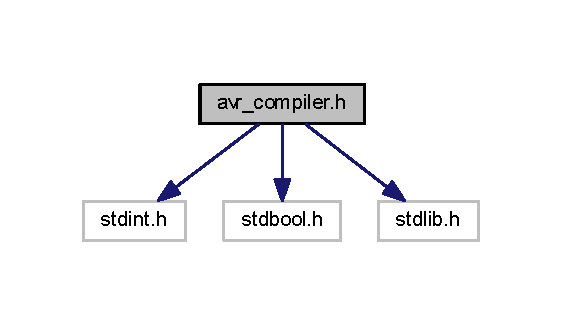
\includegraphics[width=270pt]{avr__compiler_8h__incl}
\end{center}
\end{figure}
This graph shows which files directly or indirectly include this file\+:\nopagebreak
\begin{figure}[H]
\begin{center}
\leavevmode
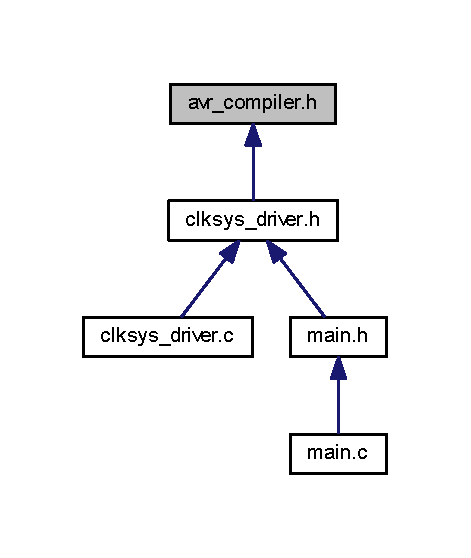
\includegraphics[width=226pt]{avr__compiler_8h__dep__incl}
\end{center}
\end{figure}
\subsection*{Macros}
\begin{DoxyCompactItemize}
\item 
\#define \hyperlink{avr__compiler_8h_a43bafb28b29491ec7f871319b5a3b2f8}{F\+\_\+\+C\+PU}~2000000\+UL
\begin{DoxyCompactList}\small\item\em Define default C\+PU frequency, if this is not already defined. \end{DoxyCompactList}\item 
\#define \hyperlink{avr__compiler_8h_a0a4fb62f9e69209c9c8c8e34ebb3df6f}{A\+V\+R\+\_\+\+E\+N\+T\+E\+R\+\_\+\+C\+R\+I\+T\+I\+C\+A\+L\+\_\+\+R\+E\+G\+I\+ON}()
\begin{DoxyCompactList}\small\item\em This macro will protect the following code from interrupts. \end{DoxyCompactList}\item 
\#define \hyperlink{avr__compiler_8h_a770b47b04eec57748be0826a3d23503b}{A\+V\+R\+\_\+\+L\+E\+A\+V\+E\+\_\+\+C\+R\+I\+T\+I\+C\+A\+L\+\_\+\+R\+E\+G\+I\+ON}()~S\+R\+EG = saved\+\_\+sreg;
\begin{DoxyCompactList}\small\item\em This macro must always be used in conjunction with A\+V\+R\+\_\+\+E\+N\+T\+E\+R\+\_\+\+C\+R\+I\+T\+I\+C\+A\+L\+\_\+\+R\+E\+G\+I\+ON so the interrupts are enabled again. \end{DoxyCompactList}\end{DoxyCompactItemize}


\subsection{Detailed Description}
This file implements some macros that makes the I\+AR C-\/compiler and avr-\/gcc work with the same code base for the A\+VR architecture. 

\begin{DoxyParagraph}{Documentation}
For comprehensive code documentation, supported compilers, compiler settings and supported devices see readme.\+html
\end{DoxyParagraph}
\begin{DoxyAuthor}{Author}
Atmel Corporation\+: \href{http://www.atmel.com}{\tt http\+://www.\+atmel.\+com} ~\newline
 Support email\+: \href{mailto:avr@atmel.com}{\tt avr@atmel.\+com}
\end{DoxyAuthor}
\begin{DoxyParagraph}{Revision}
2772 
\end{DoxyParagraph}
\begin{DoxyParagraph}{Date}
2009-\/09-\/11 12\+:40\+:26 +0200 (fr, 11 sep 2009) 
\end{DoxyParagraph}
~\newline
 Copyright (c) 2008, Atmel Corporation All rights reserved.

Redistribution and use in source and binary forms, with or without modification, are permitted provided that the following conditions are met\+:


\begin{DoxyEnumerate}
\item Redistributions of source code must retain the above copyright notice, this list of conditions and the following disclaimer.
\item Redistributions in binary form must reproduce the above copyright notice, this list of conditions and the following disclaimer in the documentation and/or other materials provided with the distribution.
\item The name of A\+T\+M\+EL may not be used to endorse or promote products derived from this software without specific prior written permission.
\end{DoxyEnumerate}

T\+H\+IS S\+O\+F\+T\+W\+A\+RE IS P\+R\+O\+V\+I\+D\+ED BY A\+T\+M\+EL \char`\"{}\+A\+S I\+S\char`\"{} A\+ND A\+NY E\+X\+P\+R\+E\+SS OR I\+M\+P\+L\+I\+ED W\+A\+R\+R\+A\+N\+T\+I\+ES, I\+N\+C\+L\+U\+D\+I\+NG, B\+UT N\+OT L\+I\+M\+I\+T\+ED TO, T\+HE I\+M\+P\+L\+I\+ED W\+A\+R\+R\+A\+N\+T\+I\+ES OF M\+E\+R\+C\+H\+A\+N\+T\+A\+B\+I\+L\+I\+TY A\+ND F\+I\+T\+N\+E\+SS F\+OR A P\+A\+R\+T\+I\+C\+U\+L\+AR P\+U\+R\+P\+O\+SE A\+RE E\+X\+P\+R\+E\+S\+S\+LY A\+ND S\+P\+E\+C\+I\+F\+I\+C\+A\+L\+LY D\+I\+S\+C\+L\+A\+I\+M\+ED. IN NO E\+V\+E\+NT S\+H\+A\+LL A\+T\+M\+EL BE L\+I\+A\+B\+LE F\+OR A\+NY D\+I\+R\+E\+CT, I\+N\+D\+I\+R\+E\+CT, I\+N\+C\+I\+D\+E\+N\+T\+AL, S\+P\+E\+C\+I\+AL, E\+X\+E\+M\+P\+L\+A\+RY, OR C\+O\+N\+S\+E\+Q\+U\+E\+N\+T\+I\+AL D\+A\+M\+A\+G\+ES (I\+N\+C\+L\+U\+D\+I\+NG, B\+UT N\+OT L\+I\+M\+I\+T\+ED TO, P\+R\+O\+C\+U\+R\+E\+M\+E\+NT OF S\+U\+B\+S\+T\+I\+T\+U\+TE G\+O\+O\+DS OR S\+E\+R\+V\+I\+C\+ES; L\+O\+SS OF U\+SE, D\+A\+TA, OR P\+R\+O\+F\+I\+TS; OR B\+U\+S\+I\+N\+E\+SS I\+N\+T\+E\+R\+R\+U\+P\+T\+I\+ON) H\+O\+W\+E\+V\+ER C\+A\+U\+S\+ED A\+ND ON A\+NY T\+H\+E\+O\+RY OF L\+I\+A\+B\+I\+L\+I\+TY, W\+H\+E\+T\+H\+ER IN C\+O\+N\+T\+R\+A\+CT, S\+T\+R\+I\+CT L\+I\+A\+B\+I\+L\+I\+TY, OR T\+O\+RT (I\+N\+C\+L\+U\+D\+I\+NG N\+E\+G\+L\+I\+G\+E\+N\+CE OR O\+T\+H\+E\+R\+W\+I\+SE) A\+R\+I\+S\+I\+NG IN A\+NY W\+AY O\+UT OF T\+HE U\+SE OF T\+H\+IS S\+O\+F\+T\+W\+A\+RE, E\+V\+EN IF A\+D\+V\+I\+S\+ED OF T\+HE P\+O\+S\+S\+I\+B\+I\+L\+I\+TY OF S\+U\+CH D\+A\+M\+A\+GE. 

\subsection{Macro Definition Documentation}
\hypertarget{avr__compiler_8h_a0a4fb62f9e69209c9c8c8e34ebb3df6f}{}\label{avr__compiler_8h_a0a4fb62f9e69209c9c8c8e34ebb3df6f} 
\index{avr\+\_\+compiler.\+h@{avr\+\_\+compiler.\+h}!A\+V\+R\+\_\+\+E\+N\+T\+E\+R\+\_\+\+C\+R\+I\+T\+I\+C\+A\+L\+\_\+\+R\+E\+G\+I\+ON@{A\+V\+R\+\_\+\+E\+N\+T\+E\+R\+\_\+\+C\+R\+I\+T\+I\+C\+A\+L\+\_\+\+R\+E\+G\+I\+ON}}
\index{A\+V\+R\+\_\+\+E\+N\+T\+E\+R\+\_\+\+C\+R\+I\+T\+I\+C\+A\+L\+\_\+\+R\+E\+G\+I\+ON@{A\+V\+R\+\_\+\+E\+N\+T\+E\+R\+\_\+\+C\+R\+I\+T\+I\+C\+A\+L\+\_\+\+R\+E\+G\+I\+ON}!avr\+\_\+compiler.\+h@{avr\+\_\+compiler.\+h}}
\subsubsection{\texorpdfstring{A\+V\+R\+\_\+\+E\+N\+T\+E\+R\+\_\+\+C\+R\+I\+T\+I\+C\+A\+L\+\_\+\+R\+E\+G\+I\+ON}{AVR\_ENTER\_CRITICAL\_REGION}}
{\footnotesize\ttfamily \#define A\+V\+R\+\_\+\+E\+N\+T\+E\+R\+\_\+\+C\+R\+I\+T\+I\+C\+A\+L\+\_\+\+R\+E\+G\+I\+ON(\begin{DoxyParamCaption}{ }\end{DoxyParamCaption})}

{\bfseries Value\+:}
\begin{DoxyCode}
uint8\_t \textcolor{keyword}{volatile} saved\_sreg = SREG; \(\backslash\)
                                     cli();
\end{DoxyCode}


This macro will protect the following code from interrupts. 



Definition at line 58 of file avr\+\_\+compiler.\+h.



Referenced by C\+C\+P\+Write().

\hypertarget{avr__compiler_8h_a770b47b04eec57748be0826a3d23503b}{}\label{avr__compiler_8h_a770b47b04eec57748be0826a3d23503b} 
\index{avr\+\_\+compiler.\+h@{avr\+\_\+compiler.\+h}!A\+V\+R\+\_\+\+L\+E\+A\+V\+E\+\_\+\+C\+R\+I\+T\+I\+C\+A\+L\+\_\+\+R\+E\+G\+I\+ON@{A\+V\+R\+\_\+\+L\+E\+A\+V\+E\+\_\+\+C\+R\+I\+T\+I\+C\+A\+L\+\_\+\+R\+E\+G\+I\+ON}}
\index{A\+V\+R\+\_\+\+L\+E\+A\+V\+E\+\_\+\+C\+R\+I\+T\+I\+C\+A\+L\+\_\+\+R\+E\+G\+I\+ON@{A\+V\+R\+\_\+\+L\+E\+A\+V\+E\+\_\+\+C\+R\+I\+T\+I\+C\+A\+L\+\_\+\+R\+E\+G\+I\+ON}!avr\+\_\+compiler.\+h@{avr\+\_\+compiler.\+h}}
\subsubsection{\texorpdfstring{A\+V\+R\+\_\+\+L\+E\+A\+V\+E\+\_\+\+C\+R\+I\+T\+I\+C\+A\+L\+\_\+\+R\+E\+G\+I\+ON}{AVR\_LEAVE\_CRITICAL\_REGION}}
{\footnotesize\ttfamily \#define A\+V\+R\+\_\+\+L\+E\+A\+V\+E\+\_\+\+C\+R\+I\+T\+I\+C\+A\+L\+\_\+\+R\+E\+G\+I\+ON(\begin{DoxyParamCaption}{ }\end{DoxyParamCaption})~S\+R\+EG = saved\+\_\+sreg;}



This macro must always be used in conjunction with A\+V\+R\+\_\+\+E\+N\+T\+E\+R\+\_\+\+C\+R\+I\+T\+I\+C\+A\+L\+\_\+\+R\+E\+G\+I\+ON so the interrupts are enabled again. 



Definition at line 64 of file avr\+\_\+compiler.\+h.



Referenced by C\+C\+P\+Write().

\hypertarget{avr__compiler_8h_a43bafb28b29491ec7f871319b5a3b2f8}{}\label{avr__compiler_8h_a43bafb28b29491ec7f871319b5a3b2f8} 
\index{avr\+\_\+compiler.\+h@{avr\+\_\+compiler.\+h}!F\+\_\+\+C\+PU@{F\+\_\+\+C\+PU}}
\index{F\+\_\+\+C\+PU@{F\+\_\+\+C\+PU}!avr\+\_\+compiler.\+h@{avr\+\_\+compiler.\+h}}
\subsubsection{\texorpdfstring{F\+\_\+\+C\+PU}{F\_CPU}}
{\footnotesize\ttfamily \#define F\+\_\+\+C\+PU~2000000\+UL}



Define default C\+PU frequency, if this is not already defined. 



Definition at line 50 of file avr\+\_\+compiler.\+h.


\hypertarget{clksys__driver_8c}{}\section{clksys\+\_\+driver.\+c File Reference}
\label{clksys__driver_8c}\index{clksys\+\_\+driver.\+c@{clksys\+\_\+driver.\+c}}


X\+M\+E\+GA Clock System driver source file.  


{\ttfamily \#include \char`\"{}clksys\+\_\+driver.\+h\char`\"{}}\newline
Include dependency graph for clksys\+\_\+driver.\+c\+:\nopagebreak
\begin{figure}[H]
\begin{center}
\leavevmode
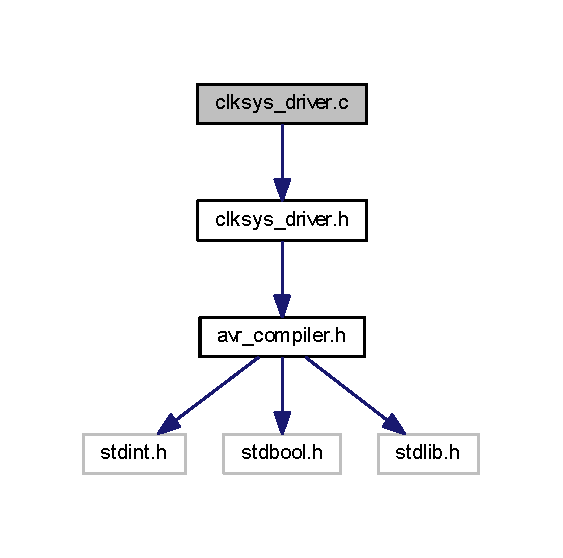
\includegraphics[width=270pt]{clksys__driver_8c__incl}
\end{center}
\end{figure}
\subsection*{Functions}
\begin{DoxyCompactItemize}
\item 
void \hyperlink{clksys__driver_8c_aad4e162434c2cc7e0087bbc0ddfe266c}{C\+C\+P\+Write} (volatile uint8\+\_\+t $\ast$address, uint8\+\_\+t value)
\begin{DoxyCompactList}\small\item\em C\+CP write helper function written in assembly. \end{DoxyCompactList}\item 
void \hyperlink{clksys__driver_8c_ace371b352e90117520436eb125aeeec0}{C\+L\+K\+S\+Y\+S\+\_\+\+X\+O\+S\+C\+\_\+\+Config} (O\+S\+C\+\_\+\+F\+R\+Q\+R\+A\+N\+G\+E\+\_\+t freq\+Range, bool low\+Power32k\+Hz, O\+S\+C\+\_\+\+X\+O\+S\+C\+S\+E\+L\+\_\+t xosc\+Mode\+Selection)
\begin{DoxyCompactList}\small\item\em This function configures the external oscillator. \end{DoxyCompactList}\item 
void \hyperlink{clksys__driver_8c_acb82744003806825da7fb6a7bb973941}{C\+L\+K\+S\+Y\+S\+\_\+\+P\+L\+L\+\_\+\+Config} (O\+S\+C\+\_\+\+P\+L\+L\+S\+R\+C\+\_\+t clock\+Source, uint8\+\_\+t factor)
\begin{DoxyCompactList}\small\item\em This function configures the internal high-\/frequency P\+LL. \end{DoxyCompactList}\item 
uint8\+\_\+t \hyperlink{clksys__driver_8c_a31b1ca1994b6a687974a119d1ad8008c}{C\+L\+K\+S\+Y\+S\+\_\+\+Disable} (uint8\+\_\+t osc\+Sel)
\begin{DoxyCompactList}\small\item\em This function disables the selected oscillator. \end{DoxyCompactList}\item 
void \hyperlink{clksys__driver_8c_a8e350b689dc409a4c9b902a192d1e8a3}{C\+L\+K\+S\+Y\+S\+\_\+\+Prescalers\+\_\+\+Config} (C\+L\+K\+\_\+\+P\+S\+A\+D\+I\+V\+\_\+t P\+S\+Afactor, C\+L\+K\+\_\+\+P\+S\+B\+C\+D\+I\+V\+\_\+t P\+S\+B\+Cfactor)
\begin{DoxyCompactList}\small\item\em This function changes the prescaler configuration. \end{DoxyCompactList}\item 
uint8\+\_\+t \hyperlink{clksys__driver_8c_a1e46c4a8f01a83d4e4747d32d113e7e2}{C\+L\+K\+S\+Y\+S\+\_\+\+Main\+\_\+\+Clock\+Source\+\_\+\+Select} (C\+L\+K\+\_\+\+S\+C\+L\+K\+S\+E\+L\+\_\+t clock\+Source)
\begin{DoxyCompactList}\small\item\em This function selects the main system clock source. \end{DoxyCompactList}\item 
void \hyperlink{clksys__driver_8c_ae622e3056cd713fdca464b9fd6e5a7ab}{C\+L\+K\+S\+Y\+S\+\_\+\+R\+T\+C\+\_\+\+Clock\+Source\+\_\+\+Enable} (C\+L\+K\+\_\+\+R\+T\+C\+S\+R\+C\+\_\+t clock\+Source)
\begin{DoxyCompactList}\small\item\em This function selects a Real-\/\+Time Counter clock source. \end{DoxyCompactList}\item 
void \hyperlink{clksys__driver_8c_a581c15c6c0b2eaa0c81f0b5cafc3b82d}{C\+L\+K\+S\+Y\+S\+\_\+\+Auto\+Calibration\+\_\+\+Enable} (uint8\+\_\+t clk\+Source, bool ext\+Reference)
\begin{DoxyCompactList}\small\item\em This function enables automatic calibration of the selected internal oscillator. \end{DoxyCompactList}\item 
void \hyperlink{clksys__driver_8c_abfb0da2d81736412af825d46e7e0cedb}{C\+L\+K\+S\+Y\+S\+\_\+\+X\+O\+S\+C\+\_\+\+Failure\+Detection\+\_\+\+Enable} (void)
\begin{DoxyCompactList}\small\item\em This function enables the External Oscillator Failure Detection (X\+O\+S\+C\+FD) feature. \end{DoxyCompactList}\item 
void \hyperlink{clksys__driver_8c_a6225fea8fc405c6d1dab88d0ad537173}{C\+L\+K\+S\+Y\+S\+\_\+\+Configuration\+\_\+\+Lock} (void)
\begin{DoxyCompactList}\small\item\em This function lock the entire clock system configuration. \end{DoxyCompactList}\end{DoxyCompactItemize}


\subsection{Detailed Description}
X\+M\+E\+GA Clock System driver source file. 

This file contains the function implementations for the X\+M\+E\+GA Clock System driver.

The driver is not intended for size and/or speed critical code, since most functions are just a few lines of code, and the function call overhead would decrease code performance. The driver is intended for rapid prototyping and documentation purposes for getting started with the X\+M\+E\+GA Clock System.

For size and/or speed critical code, it is recommended to copy the function contents directly into your application instead of making a function call.

Several functions use the following construct\+: \char`\"{}some\+\_\+register = ... $\vert$ (some\+\_\+parameter ? S\+O\+M\+E\+\_\+\+B\+I\+T\+\_\+bm \+: 0) $\vert$ ...\char`\"{} Although the use of the ternary operator ( if ? then \+: else ) is discouraged, in some occasions the operator makes it possible to write pretty clean and neat code. In this driver, the construct is used to set or not set a configuration bit based on a boolean input parameter, such as the \char`\"{}some\+\_\+parameter\char`\"{} in the example above.

\begin{DoxyParagraph}{Application note\+:}
A\+V\+R1003\+: Using the X\+M\+E\+GA Clock System
\end{DoxyParagraph}
\begin{DoxyParagraph}{Documentation}
For comprehensive code documentation, supported compilers, compiler settings and supported devices see readme.\+html
\end{DoxyParagraph}
\begin{DoxyAuthor}{Author}
Atmel Corporation\+: \href{http://www.atmel.com}{\tt http\+://www.\+atmel.\+com} ~\newline
 Support email\+: \href{mailto:avr@atmel.com}{\tt avr@atmel.\+com}
\end{DoxyAuthor}
\begin{DoxyParagraph}{Revision}
2771 
\end{DoxyParagraph}
\begin{DoxyParagraph}{Date}
2009-\/09-\/11 11\+:54\+:26 +0200 (fr, 11 sep 2009) 
\end{DoxyParagraph}
~\newline
 Copyright (c) 2008, Atmel Corporation All rights reserved.

Redistribution and use in source and binary forms, with or without modification, are permitted provided that the following conditions are met\+:


\begin{DoxyEnumerate}
\item Redistributions of source code must retain the above copyright notice, this list of conditions and the following disclaimer.
\item Redistributions in binary form must reproduce the above copyright notice, this list of conditions and the following disclaimer in the documentation and/or other materials provided with the distribution.
\item The name of A\+T\+M\+EL may not be used to endorse or promote products derived from this software without specific prior written permission.
\end{DoxyEnumerate}

T\+H\+IS S\+O\+F\+T\+W\+A\+RE IS P\+R\+O\+V\+I\+D\+ED BY A\+T\+M\+EL \char`\"{}\+A\+S I\+S\char`\"{} A\+ND A\+NY E\+X\+P\+R\+E\+SS OR I\+M\+P\+L\+I\+ED W\+A\+R\+R\+A\+N\+T\+I\+ES, I\+N\+C\+L\+U\+D\+I\+NG, B\+UT N\+OT L\+I\+M\+I\+T\+ED TO, T\+HE I\+M\+P\+L\+I\+ED W\+A\+R\+R\+A\+N\+T\+I\+ES OF M\+E\+R\+C\+H\+A\+N\+T\+A\+B\+I\+L\+I\+TY A\+ND F\+I\+T\+N\+E\+SS F\+OR A P\+A\+R\+T\+I\+C\+U\+L\+AR P\+U\+R\+P\+O\+SE A\+RE E\+X\+P\+R\+E\+S\+S\+LY A\+ND S\+P\+E\+C\+I\+F\+I\+C\+A\+L\+LY D\+I\+S\+C\+L\+A\+I\+M\+ED. IN NO E\+V\+E\+NT S\+H\+A\+LL A\+T\+M\+EL BE L\+I\+A\+B\+LE F\+OR A\+NY D\+I\+R\+E\+CT, I\+N\+D\+I\+R\+E\+CT, I\+N\+C\+I\+D\+E\+N\+T\+AL, S\+P\+E\+C\+I\+AL, E\+X\+E\+M\+P\+L\+A\+RY, OR C\+O\+N\+S\+E\+Q\+U\+E\+N\+T\+I\+AL D\+A\+M\+A\+G\+ES (I\+N\+C\+L\+U\+D\+I\+NG, B\+UT N\+OT L\+I\+M\+I\+T\+ED TO, P\+R\+O\+C\+U\+R\+E\+M\+E\+NT OF S\+U\+B\+S\+T\+I\+T\+U\+TE G\+O\+O\+DS OR S\+E\+R\+V\+I\+C\+ES; L\+O\+SS OF U\+SE, D\+A\+TA, OR P\+R\+O\+F\+I\+TS; OR B\+U\+S\+I\+N\+E\+SS I\+N\+T\+E\+R\+R\+U\+P\+T\+I\+ON) H\+O\+W\+E\+V\+ER C\+A\+U\+S\+ED A\+ND ON A\+NY T\+H\+E\+O\+RY OF L\+I\+A\+B\+I\+L\+I\+TY, W\+H\+E\+T\+H\+ER IN C\+O\+N\+T\+R\+A\+CT, S\+T\+R\+I\+CT L\+I\+A\+B\+I\+L\+I\+TY, OR T\+O\+RT (I\+N\+C\+L\+U\+D\+I\+NG N\+E\+G\+L\+I\+G\+E\+N\+CE OR O\+T\+H\+E\+R\+W\+I\+SE) A\+R\+I\+S\+I\+NG IN A\+NY W\+AY O\+UT OF T\+HE U\+SE OF T\+H\+IS S\+O\+F\+T\+W\+A\+RE, E\+V\+EN IF A\+D\+V\+I\+S\+ED OF T\+HE P\+O\+S\+S\+I\+B\+I\+L\+I\+TY OF S\+U\+CH D\+A\+M\+A\+GE. 

\subsection{Function Documentation}
\hypertarget{clksys__driver_8c_aad4e162434c2cc7e0087bbc0ddfe266c}{}\label{clksys__driver_8c_aad4e162434c2cc7e0087bbc0ddfe266c} 
\index{clksys\+\_\+driver.\+c@{clksys\+\_\+driver.\+c}!C\+C\+P\+Write@{C\+C\+P\+Write}}
\index{C\+C\+P\+Write@{C\+C\+P\+Write}!clksys\+\_\+driver.\+c@{clksys\+\_\+driver.\+c}}
\subsubsection{\texorpdfstring{C\+C\+P\+Write()}{CCPWrite()}}
{\footnotesize\ttfamily void C\+C\+P\+Write (\begin{DoxyParamCaption}\item[{volatile uint8\+\_\+t $\ast$}]{address,  }\item[{uint8\+\_\+t}]{value }\end{DoxyParamCaption})}



C\+CP write helper function written in assembly. 

This function is written in assembly because of the timecritial operation of writing to the registers.


\begin{DoxyParams}{Parameters}
{\em address} & A pointer to the address to write to. \\
\hline
{\em value} & The value to put in to the register. \\
\hline
\end{DoxyParams}


Definition at line 77 of file clksys\+\_\+driver.\+c.



References A\+V\+R\+\_\+\+E\+N\+T\+E\+R\+\_\+\+C\+R\+I\+T\+I\+C\+A\+L\+\_\+\+R\+E\+G\+I\+ON, and A\+V\+R\+\_\+\+L\+E\+A\+V\+E\+\_\+\+C\+R\+I\+T\+I\+C\+A\+L\+\_\+\+R\+E\+G\+I\+ON.



Referenced by C\+L\+K\+S\+Y\+S\+\_\+\+Configuration\+\_\+\+Lock(), C\+L\+K\+S\+Y\+S\+\_\+\+Main\+\_\+\+Clock\+Source\+\_\+\+Select(), C\+L\+K\+S\+Y\+S\+\_\+\+Prescalers\+\_\+\+Config(), and C\+L\+K\+S\+Y\+S\+\_\+\+X\+O\+S\+C\+\_\+\+Failure\+Detection\+\_\+\+Enable().

Here is the caller graph for this function\+:\nopagebreak
\begin{figure}[H]
\begin{center}
\leavevmode
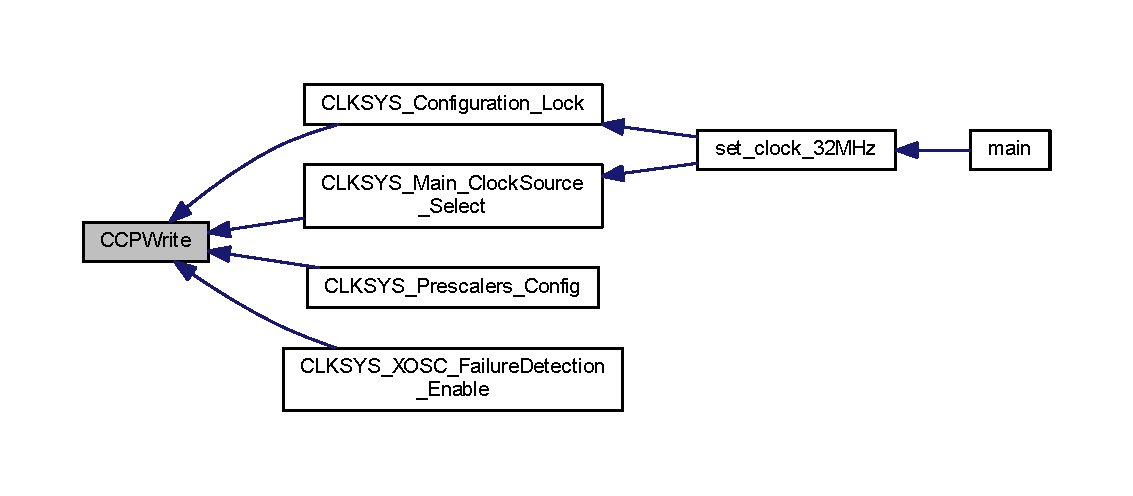
\includegraphics[width=350pt]{clksys__driver_8c_aad4e162434c2cc7e0087bbc0ddfe266c_icgraph}
\end{center}
\end{figure}
\hypertarget{clksys__driver_8c_a581c15c6c0b2eaa0c81f0b5cafc3b82d}{}\label{clksys__driver_8c_a581c15c6c0b2eaa0c81f0b5cafc3b82d} 
\index{clksys\+\_\+driver.\+c@{clksys\+\_\+driver.\+c}!C\+L\+K\+S\+Y\+S\+\_\+\+Auto\+Calibration\+\_\+\+Enable@{C\+L\+K\+S\+Y\+S\+\_\+\+Auto\+Calibration\+\_\+\+Enable}}
\index{C\+L\+K\+S\+Y\+S\+\_\+\+Auto\+Calibration\+\_\+\+Enable@{C\+L\+K\+S\+Y\+S\+\_\+\+Auto\+Calibration\+\_\+\+Enable}!clksys\+\_\+driver.\+c@{clksys\+\_\+driver.\+c}}
\subsubsection{\texorpdfstring{C\+L\+K\+S\+Y\+S\+\_\+\+Auto\+Calibration\+\_\+\+Enable()}{CLKSYS\_AutoCalibration\_Enable()}}
{\footnotesize\ttfamily void C\+L\+K\+S\+Y\+S\+\_\+\+Auto\+Calibration\+\_\+\+Enable (\begin{DoxyParamCaption}\item[{uint8\+\_\+t}]{clk\+Source,  }\item[{bool}]{ext\+Reference }\end{DoxyParamCaption})}



This function enables automatic calibration of the selected internal oscillator. 

Either the internal 32k\+Hz RC oscillator or an external 32k\+Hz crystal can be used as a calibration reference. The user must make sure that the selected reference is ready and running.


\begin{DoxyParams}{Parameters}
{\em clk\+Source} & Clock source to calibrate, either O\+S\+C\+\_\+\+R\+C2\+M\+C\+R\+E\+F\+\_\+bm or O\+S\+C\+\_\+\+R\+C32\+M\+C\+R\+E\+F\+\_\+gm -\/ patched to group mask(jb). \\
\hline
{\em ext\+Reference} & True if external crystal should be used as reference. \\
\hline
\end{DoxyParams}


Definition at line 260 of file clksys\+\_\+driver.\+c.



Referenced by set\+\_\+clock\+\_\+32\+M\+Hz().

Here is the caller graph for this function\+:\nopagebreak
\begin{figure}[H]
\begin{center}
\leavevmode
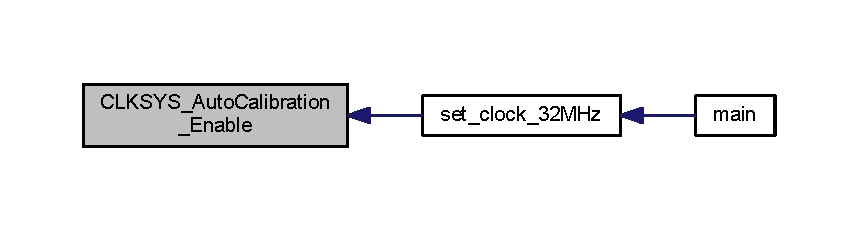
\includegraphics[width=350pt]{clksys__driver_8c_a581c15c6c0b2eaa0c81f0b5cafc3b82d_icgraph}
\end{center}
\end{figure}
\hypertarget{clksys__driver_8c_a6225fea8fc405c6d1dab88d0ad537173}{}\label{clksys__driver_8c_a6225fea8fc405c6d1dab88d0ad537173} 
\index{clksys\+\_\+driver.\+c@{clksys\+\_\+driver.\+c}!C\+L\+K\+S\+Y\+S\+\_\+\+Configuration\+\_\+\+Lock@{C\+L\+K\+S\+Y\+S\+\_\+\+Configuration\+\_\+\+Lock}}
\index{C\+L\+K\+S\+Y\+S\+\_\+\+Configuration\+\_\+\+Lock@{C\+L\+K\+S\+Y\+S\+\_\+\+Configuration\+\_\+\+Lock}!clksys\+\_\+driver.\+c@{clksys\+\_\+driver.\+c}}
\subsubsection{\texorpdfstring{C\+L\+K\+S\+Y\+S\+\_\+\+Configuration\+\_\+\+Lock()}{CLKSYS\_Configuration\_Lock()}}
{\footnotesize\ttfamily void C\+L\+K\+S\+Y\+S\+\_\+\+Configuration\+\_\+\+Lock (\begin{DoxyParamCaption}\item[{void}]{ }\end{DoxyParamCaption})}



This function lock the entire clock system configuration. 

This will lock the configuration until the next reset, or until the External Oscillator Failure Detections (X\+O\+S\+C\+FD) feature detects a failure and switches to internal 2\+M\+Hz RC oscillator. 

Definition at line 292 of file clksys\+\_\+driver.\+c.



References C\+C\+P\+Write().



Referenced by set\+\_\+clock\+\_\+32\+M\+Hz().

Here is the call graph for this function\+:\nopagebreak
\begin{figure}[H]
\begin{center}
\leavevmode
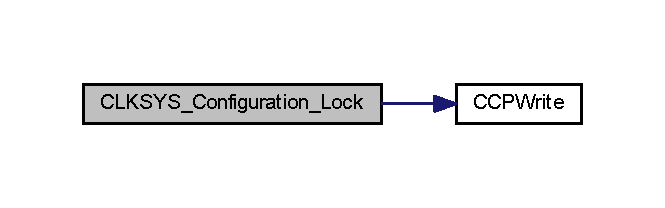
\includegraphics[width=319pt]{clksys__driver_8c_a6225fea8fc405c6d1dab88d0ad537173_cgraph}
\end{center}
\end{figure}
Here is the caller graph for this function\+:\nopagebreak
\begin{figure}[H]
\begin{center}
\leavevmode
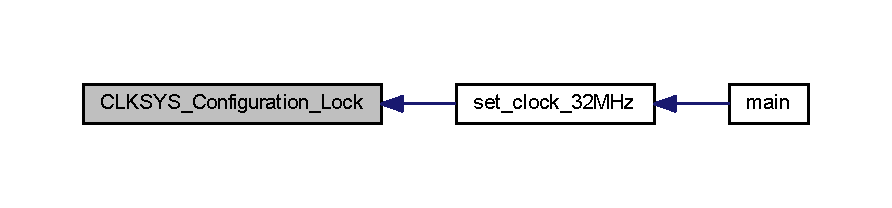
\includegraphics[width=350pt]{clksys__driver_8c_a6225fea8fc405c6d1dab88d0ad537173_icgraph}
\end{center}
\end{figure}
\hypertarget{clksys__driver_8c_a31b1ca1994b6a687974a119d1ad8008c}{}\label{clksys__driver_8c_a31b1ca1994b6a687974a119d1ad8008c} 
\index{clksys\+\_\+driver.\+c@{clksys\+\_\+driver.\+c}!C\+L\+K\+S\+Y\+S\+\_\+\+Disable@{C\+L\+K\+S\+Y\+S\+\_\+\+Disable}}
\index{C\+L\+K\+S\+Y\+S\+\_\+\+Disable@{C\+L\+K\+S\+Y\+S\+\_\+\+Disable}!clksys\+\_\+driver.\+c@{clksys\+\_\+driver.\+c}}
\subsubsection{\texorpdfstring{C\+L\+K\+S\+Y\+S\+\_\+\+Disable()}{CLKSYS\_Disable()}}
{\footnotesize\ttfamily uint8\+\_\+t C\+L\+K\+S\+Y\+S\+\_\+\+Disable (\begin{DoxyParamCaption}\item[{uint8\+\_\+t}]{osc\+Sel }\end{DoxyParamCaption})}



This function disables the selected oscillator. 

This function will disable the selected oscillator if possible. If it is currently used as a main system clock source, hardware will disregard the disable attempt, and this function will return zero. If it fails, change to another main system clock source and try again.


\begin{DoxyParams}{Parameters}
{\em osc\+Sel} & Bitmask of selected clock. Can be one of the following O\+S\+C\+\_\+\+R\+C2\+M\+E\+N\+\_\+bm, O\+S\+C\+\_\+\+R\+C32\+M\+E\+N\+\_\+bm, O\+S\+C\+\_\+\+R\+C32\+K\+E\+N\+\_\+bm, O\+S\+C\+\_\+\+X\+O\+S\+C\+E\+N\+\_\+bm, O\+S\+C\+\_\+\+P\+L\+L\+E\+N\+\_\+bm.\\
\hline
\end{DoxyParams}
\begin{DoxyReturn}{Returns}
Non-\/zero if oscillator was disabled successfully. 
\end{DoxyReturn}


Definition at line 187 of file clksys\+\_\+driver.\+c.



Referenced by set\+\_\+clock\+\_\+32\+M\+Hz().

Here is the caller graph for this function\+:\nopagebreak
\begin{figure}[H]
\begin{center}
\leavevmode
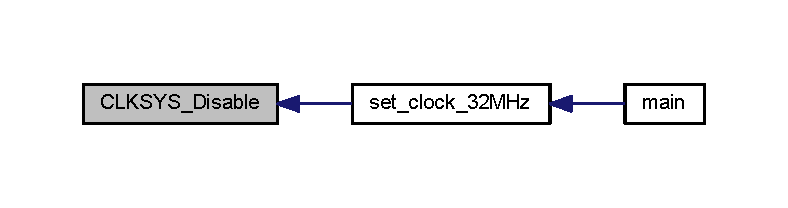
\includegraphics[width=350pt]{clksys__driver_8c_a31b1ca1994b6a687974a119d1ad8008c_icgraph}
\end{center}
\end{figure}
\hypertarget{clksys__driver_8c_a1e46c4a8f01a83d4e4747d32d113e7e2}{}\label{clksys__driver_8c_a1e46c4a8f01a83d4e4747d32d113e7e2} 
\index{clksys\+\_\+driver.\+c@{clksys\+\_\+driver.\+c}!C\+L\+K\+S\+Y\+S\+\_\+\+Main\+\_\+\+Clock\+Source\+\_\+\+Select@{C\+L\+K\+S\+Y\+S\+\_\+\+Main\+\_\+\+Clock\+Source\+\_\+\+Select}}
\index{C\+L\+K\+S\+Y\+S\+\_\+\+Main\+\_\+\+Clock\+Source\+\_\+\+Select@{C\+L\+K\+S\+Y\+S\+\_\+\+Main\+\_\+\+Clock\+Source\+\_\+\+Select}!clksys\+\_\+driver.\+c@{clksys\+\_\+driver.\+c}}
\subsubsection{\texorpdfstring{C\+L\+K\+S\+Y\+S\+\_\+\+Main\+\_\+\+Clock\+Source\+\_\+\+Select()}{CLKSYS\_Main\_ClockSource\_Select()}}
{\footnotesize\ttfamily uint8\+\_\+t C\+L\+K\+S\+Y\+S\+\_\+\+Main\+\_\+\+Clock\+Source\+\_\+\+Select (\begin{DoxyParamCaption}\item[{C\+L\+K\+\_\+\+S\+C\+L\+K\+S\+E\+L\+\_\+t}]{clock\+Source }\end{DoxyParamCaption})}



This function selects the main system clock source. 

Hardware will disregard any attempts to select a clock source that is not enabled or not stable. If the change fails, make sure the source is ready and running and try again.


\begin{DoxyParams}{Parameters}
{\em clock\+Source} & Clock source to use as input for the system clock prescaler block.\\
\hline
\end{DoxyParams}
\begin{DoxyReturn}{Returns}
Non-\/zero if change was successful. 
\end{DoxyReturn}


Definition at line 225 of file clksys\+\_\+driver.\+c.



References C\+C\+P\+Write().



Referenced by set\+\_\+clock\+\_\+32\+M\+Hz().

Here is the call graph for this function\+:\nopagebreak
\begin{figure}[H]
\begin{center}
\leavevmode
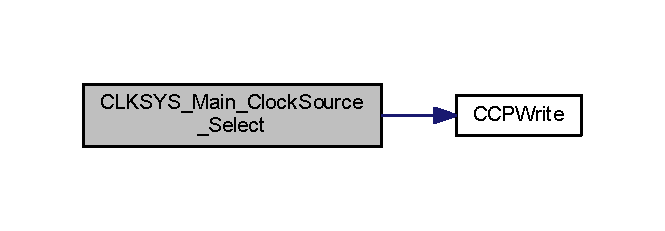
\includegraphics[width=319pt]{clksys__driver_8c_a1e46c4a8f01a83d4e4747d32d113e7e2_cgraph}
\end{center}
\end{figure}
Here is the caller graph for this function\+:\nopagebreak
\begin{figure}[H]
\begin{center}
\leavevmode
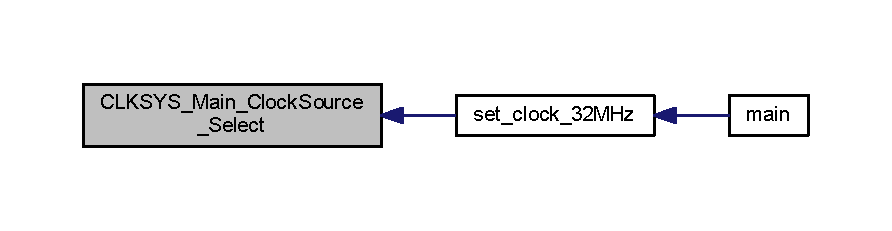
\includegraphics[width=350pt]{clksys__driver_8c_a1e46c4a8f01a83d4e4747d32d113e7e2_icgraph}
\end{center}
\end{figure}
\hypertarget{clksys__driver_8c_acb82744003806825da7fb6a7bb973941}{}\label{clksys__driver_8c_acb82744003806825da7fb6a7bb973941} 
\index{clksys\+\_\+driver.\+c@{clksys\+\_\+driver.\+c}!C\+L\+K\+S\+Y\+S\+\_\+\+P\+L\+L\+\_\+\+Config@{C\+L\+K\+S\+Y\+S\+\_\+\+P\+L\+L\+\_\+\+Config}}
\index{C\+L\+K\+S\+Y\+S\+\_\+\+P\+L\+L\+\_\+\+Config@{C\+L\+K\+S\+Y\+S\+\_\+\+P\+L\+L\+\_\+\+Config}!clksys\+\_\+driver.\+c@{clksys\+\_\+driver.\+c}}
\subsubsection{\texorpdfstring{C\+L\+K\+S\+Y\+S\+\_\+\+P\+L\+L\+\_\+\+Config()}{CLKSYS\_PLL\_Config()}}
{\footnotesize\ttfamily void C\+L\+K\+S\+Y\+S\+\_\+\+P\+L\+L\+\_\+\+Config (\begin{DoxyParamCaption}\item[{O\+S\+C\+\_\+\+P\+L\+L\+S\+R\+C\+\_\+t}]{clock\+Source,  }\item[{uint8\+\_\+t}]{factor }\end{DoxyParamCaption})}



This function configures the internal high-\/frequency P\+LL. 

Configuration of the internal high-\/frequency P\+LL to the correct values. It is used to define the input of the P\+LL and the factor of multiplication of the input clock source.

\begin{DoxyNote}{Note}
Note that the oscillator cannot be used as a main system clock source without being enabled and stable first. Check the ready flag before using the clock. The macro \hyperlink{clksys__driver_8h_a2cd92dbb89e4051b9385a61273d19dc6}{C\+L\+K\+S\+Y\+S\+\_\+\+Is\+Ready( \+\_\+osc\+Sel )} can be used to check this.
\end{DoxyNote}

\begin{DoxyParams}{Parameters}
{\em clock\+Source} & Reference clock source for the P\+LL, must be above 0.\+4\+M\+Hz. \\
\hline
{\em factor} & P\+LL multiplication factor, must be from 1 to 31, inclusive. \\
\hline
\end{DoxyParams}


Definition at line 167 of file clksys\+\_\+driver.\+c.

\hypertarget{clksys__driver_8c_a8e350b689dc409a4c9b902a192d1e8a3}{}\label{clksys__driver_8c_a8e350b689dc409a4c9b902a192d1e8a3} 
\index{clksys\+\_\+driver.\+c@{clksys\+\_\+driver.\+c}!C\+L\+K\+S\+Y\+S\+\_\+\+Prescalers\+\_\+\+Config@{C\+L\+K\+S\+Y\+S\+\_\+\+Prescalers\+\_\+\+Config}}
\index{C\+L\+K\+S\+Y\+S\+\_\+\+Prescalers\+\_\+\+Config@{C\+L\+K\+S\+Y\+S\+\_\+\+Prescalers\+\_\+\+Config}!clksys\+\_\+driver.\+c@{clksys\+\_\+driver.\+c}}
\subsubsection{\texorpdfstring{C\+L\+K\+S\+Y\+S\+\_\+\+Prescalers\+\_\+\+Config()}{CLKSYS\_Prescalers\_Config()}}
{\footnotesize\ttfamily void C\+L\+K\+S\+Y\+S\+\_\+\+Prescalers\+\_\+\+Config (\begin{DoxyParamCaption}\item[{C\+L\+K\+\_\+\+P\+S\+A\+D\+I\+V\+\_\+t}]{P\+S\+Afactor,  }\item[{C\+L\+K\+\_\+\+P\+S\+B\+C\+D\+I\+V\+\_\+t}]{P\+S\+B\+Cfactor }\end{DoxyParamCaption})}



This function changes the prescaler configuration. 

Change the configuration of the three system clock prescaler is one single operation. The user must make sure that the main C\+PU clock does not exceed recommended limits.


\begin{DoxyParams}{Parameters}
{\em P\+S\+Afactor} & Prescaler A division factor, O\+FF or 2 to 512 in powers of two. \\
\hline
{\em P\+S\+B\+Cfactor} & Prescaler B and C division factor, in the combination of (1,1), (1,2), (4,1) or (2,2). \\
\hline
\end{DoxyParams}


Definition at line 206 of file clksys\+\_\+driver.\+c.



References C\+C\+P\+Write().

Here is the call graph for this function\+:\nopagebreak
\begin{figure}[H]
\begin{center}
\leavevmode
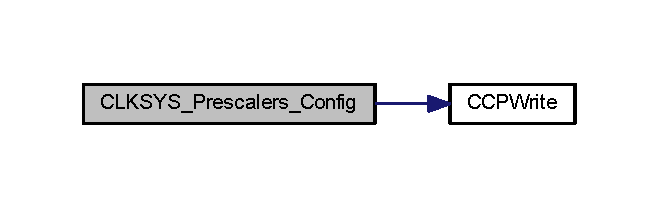
\includegraphics[width=316pt]{clksys__driver_8c_a8e350b689dc409a4c9b902a192d1e8a3_cgraph}
\end{center}
\end{figure}
\hypertarget{clksys__driver_8c_ae622e3056cd713fdca464b9fd6e5a7ab}{}\label{clksys__driver_8c_ae622e3056cd713fdca464b9fd6e5a7ab} 
\index{clksys\+\_\+driver.\+c@{clksys\+\_\+driver.\+c}!C\+L\+K\+S\+Y\+S\+\_\+\+R\+T\+C\+\_\+\+Clock\+Source\+\_\+\+Enable@{C\+L\+K\+S\+Y\+S\+\_\+\+R\+T\+C\+\_\+\+Clock\+Source\+\_\+\+Enable}}
\index{C\+L\+K\+S\+Y\+S\+\_\+\+R\+T\+C\+\_\+\+Clock\+Source\+\_\+\+Enable@{C\+L\+K\+S\+Y\+S\+\_\+\+R\+T\+C\+\_\+\+Clock\+Source\+\_\+\+Enable}!clksys\+\_\+driver.\+c@{clksys\+\_\+driver.\+c}}
\subsubsection{\texorpdfstring{C\+L\+K\+S\+Y\+S\+\_\+\+R\+T\+C\+\_\+\+Clock\+Source\+\_\+\+Enable()}{CLKSYS\_RTC\_ClockSource\_Enable()}}
{\footnotesize\ttfamily void C\+L\+K\+S\+Y\+S\+\_\+\+R\+T\+C\+\_\+\+Clock\+Source\+\_\+\+Enable (\begin{DoxyParamCaption}\item[{C\+L\+K\+\_\+\+R\+T\+C\+S\+R\+C\+\_\+t}]{clock\+Source }\end{DoxyParamCaption})}



This function selects a Real-\/\+Time Counter clock source. 

Selects the clock source for use by the Real-\/\+Time Counter (R\+TC) and enables clock signal routing to the R\+TC module.


\begin{DoxyParams}{Parameters}
{\em clock\+Source} & Clock source to use for the R\+TC. \\
\hline
\end{DoxyParams}


Definition at line 241 of file clksys\+\_\+driver.\+c.

\hypertarget{clksys__driver_8c_ace371b352e90117520436eb125aeeec0}{}\label{clksys__driver_8c_ace371b352e90117520436eb125aeeec0} 
\index{clksys\+\_\+driver.\+c@{clksys\+\_\+driver.\+c}!C\+L\+K\+S\+Y\+S\+\_\+\+X\+O\+S\+C\+\_\+\+Config@{C\+L\+K\+S\+Y\+S\+\_\+\+X\+O\+S\+C\+\_\+\+Config}}
\index{C\+L\+K\+S\+Y\+S\+\_\+\+X\+O\+S\+C\+\_\+\+Config@{C\+L\+K\+S\+Y\+S\+\_\+\+X\+O\+S\+C\+\_\+\+Config}!clksys\+\_\+driver.\+c@{clksys\+\_\+driver.\+c}}
\subsubsection{\texorpdfstring{C\+L\+K\+S\+Y\+S\+\_\+\+X\+O\+S\+C\+\_\+\+Config()}{CLKSYS\_XOSC\_Config()}}
{\footnotesize\ttfamily void C\+L\+K\+S\+Y\+S\+\_\+\+X\+O\+S\+C\+\_\+\+Config (\begin{DoxyParamCaption}\item[{O\+S\+C\+\_\+\+F\+R\+Q\+R\+A\+N\+G\+E\+\_\+t}]{freq\+Range,  }\item[{bool}]{low\+Power32k\+Hz,  }\item[{O\+S\+C\+\_\+\+X\+O\+S\+C\+S\+E\+L\+\_\+t}]{xosc\+Mode\+Selection }\end{DoxyParamCaption})}



This function configures the external oscillator. 

\begin{DoxyNote}{Note}
Note that the oscillator cannot be used as a main system clock source without being enabled and stable first. Check the ready flag before using the clock. The macro \hyperlink{clksys__driver_8h_a2cd92dbb89e4051b9385a61273d19dc6}{C\+L\+K\+S\+Y\+S\+\_\+\+Is\+Ready( \+\_\+osc\+Sel )} can be used to check this.
\end{DoxyNote}

\begin{DoxyParams}{Parameters}
{\em freq\+Range} & Frequency range for high-\/frequency crystal, does not apply for external clock or 32k\+Hz crystals. \\
\hline
{\em low\+Power32k\+Hz} & True of high-\/quality watch crystals are used and low-\/power oscillator is desired. \\
\hline
{\em xosc\+Mode\+Selection} & Combined selection of oscillator type (or external clock) and startup times. \\
\hline
\end{DoxyParams}


Definition at line 141 of file clksys\+\_\+driver.\+c.

\hypertarget{clksys__driver_8c_abfb0da2d81736412af825d46e7e0cedb}{}\label{clksys__driver_8c_abfb0da2d81736412af825d46e7e0cedb} 
\index{clksys\+\_\+driver.\+c@{clksys\+\_\+driver.\+c}!C\+L\+K\+S\+Y\+S\+\_\+\+X\+O\+S\+C\+\_\+\+Failure\+Detection\+\_\+\+Enable@{C\+L\+K\+S\+Y\+S\+\_\+\+X\+O\+S\+C\+\_\+\+Failure\+Detection\+\_\+\+Enable}}
\index{C\+L\+K\+S\+Y\+S\+\_\+\+X\+O\+S\+C\+\_\+\+Failure\+Detection\+\_\+\+Enable@{C\+L\+K\+S\+Y\+S\+\_\+\+X\+O\+S\+C\+\_\+\+Failure\+Detection\+\_\+\+Enable}!clksys\+\_\+driver.\+c@{clksys\+\_\+driver.\+c}}
\subsubsection{\texorpdfstring{C\+L\+K\+S\+Y\+S\+\_\+\+X\+O\+S\+C\+\_\+\+Failure\+Detection\+\_\+\+Enable()}{CLKSYS\_XOSC\_FailureDetection\_Enable()}}
{\footnotesize\ttfamily void C\+L\+K\+S\+Y\+S\+\_\+\+X\+O\+S\+C\+\_\+\+Failure\+Detection\+\_\+\+Enable (\begin{DoxyParamCaption}\item[{void}]{ }\end{DoxyParamCaption})}



This function enables the External Oscillator Failure Detection (X\+O\+S\+C\+FD) feature. 

The feature will stay enabled until next reset. Note that the X\+O\+S\+C\+FD {\itshape will} issue the X\+O\+S\+CF Non-\/maskable Interrupt (N\+MI) regardless of any interrupt priorities and settings. Therefore, make sure that a handler is implemented for the X\+O\+S\+CF N\+MI when you enable it. 

Definition at line 280 of file clksys\+\_\+driver.\+c.



References C\+C\+P\+Write().

Here is the call graph for this function\+:\nopagebreak
\begin{figure}[H]
\begin{center}
\leavevmode
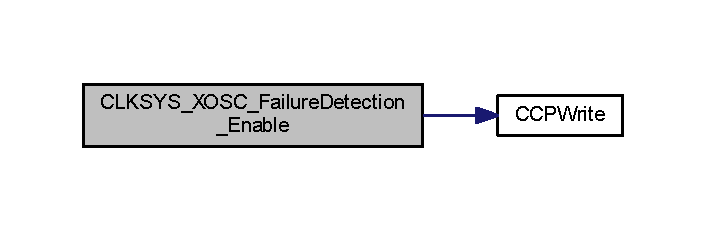
\includegraphics[width=339pt]{clksys__driver_8c_abfb0da2d81736412af825d46e7e0cedb_cgraph}
\end{center}
\end{figure}

\hypertarget{clksys__driver_8h}{}\section{clksys\+\_\+driver.\+h File Reference}
\label{clksys__driver_8h}\index{clksys\+\_\+driver.\+h@{clksys\+\_\+driver.\+h}}


X\+M\+E\+GA Clock System driver header file.  


{\ttfamily \#include \char`\"{}avr\+\_\+compiler.\+h\char`\"{}}\newline
Include dependency graph for clksys\+\_\+driver.\+h\+:\nopagebreak
\begin{figure}[H]
\begin{center}
\leavevmode
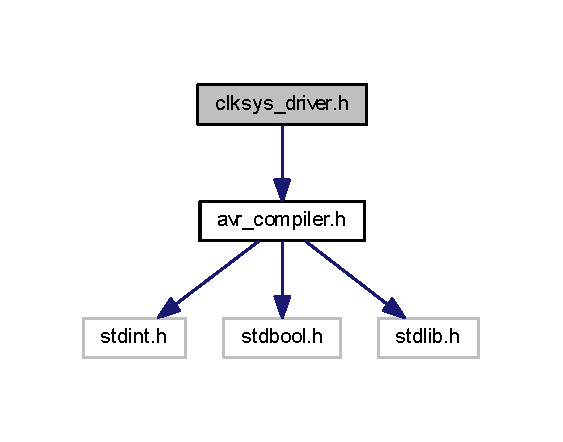
\includegraphics[width=270pt]{clksys__driver_8h__incl}
\end{center}
\end{figure}
This graph shows which files directly or indirectly include this file\+:\nopagebreak
\begin{figure}[H]
\begin{center}
\leavevmode
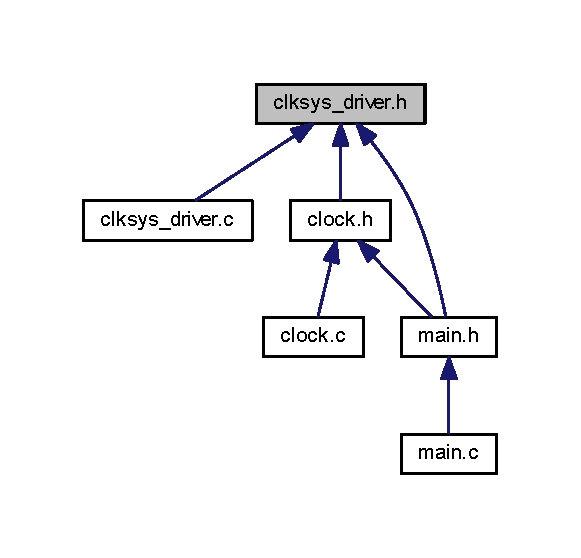
\includegraphics[width=279pt]{clksys__driver_8h__dep__incl}
\end{center}
\end{figure}
\subsection*{Macros}
\begin{DoxyCompactItemize}
\item 
\#define \hyperlink{clksys__driver_8h_a0894c64562c3b1c309bab97a83382267}{C\+L\+K\+S\+Y\+S\+\_\+\+Enable}(\+\_\+osc\+Sel)~( O\+S\+C.\+C\+T\+RL $\vert$= (\+\_\+osc\+Sel) )
\begin{DoxyCompactList}\small\item\em This macro enables the selected oscillator. \end{DoxyCompactList}\item 
\#define \hyperlink{clksys__driver_8h_a2cd92dbb89e4051b9385a61273d19dc6}{C\+L\+K\+S\+Y\+S\+\_\+\+Is\+Ready}(\+\_\+osc\+Sel)~( O\+S\+C.\+S\+T\+A\+T\+US \& (\+\_\+osc\+Sel) )
\begin{DoxyCompactList}\small\item\em This macro check if selected oscillator is ready. \end{DoxyCompactList}\item 
\#define \hyperlink{clksys__driver_8h_a2ace04e605910a306c6f65102e76c046}{C\+L\+K\+S\+Y\+S\+\_\+\+R\+T\+C\+\_\+\+Clock\+Source\+\_\+\+Disable}()~( C\+L\+K.\+R\+T\+C\+C\+T\+RL \&= $\sim$C\+L\+K\+\_\+\+R\+T\+C\+E\+N\+\_\+bm )
\begin{DoxyCompactList}\small\item\em This macro disables routing of clock signals to the Real-\/\+Time Counter (R\+TC). \end{DoxyCompactList}\item 
\#define \hyperlink{clksys__driver_8h_ab06829d3775b72351cbb2cb65dbc4dc7}{C\+L\+K\+S\+Y\+S\+\_\+\+Auto\+Calibration\+\_\+\+Disable}(\+\_\+clk)~( (\+\_\+clk).C\+T\+RL \&= $\sim$D\+F\+L\+L\+\_\+\+E\+N\+A\+B\+L\+E\+\_\+bm )
\begin{DoxyCompactList}\small\item\em This macro disables the automatic calibration of the selected internal oscillator. \end{DoxyCompactList}\end{DoxyCompactItemize}
\subsection*{Functions}
\begin{DoxyCompactItemize}
\item 
void \hyperlink{clksys__driver_8h_aad4e162434c2cc7e0087bbc0ddfe266c}{C\+C\+P\+Write} (volatile uint8\+\_\+t $\ast$address, uint8\+\_\+t value)
\begin{DoxyCompactList}\small\item\em C\+CP write helper function written in assembly. \end{DoxyCompactList}\item 
void \hyperlink{clksys__driver_8h_ace371b352e90117520436eb125aeeec0}{C\+L\+K\+S\+Y\+S\+\_\+\+X\+O\+S\+C\+\_\+\+Config} (O\+S\+C\+\_\+\+F\+R\+Q\+R\+A\+N\+G\+E\+\_\+t freq\+Range, bool low\+Power32k\+Hz, O\+S\+C\+\_\+\+X\+O\+S\+C\+S\+E\+L\+\_\+t xosc\+Mode\+Selection)
\begin{DoxyCompactList}\small\item\em This function configures the external oscillator. \end{DoxyCompactList}\item 
void \hyperlink{clksys__driver_8h_acb82744003806825da7fb6a7bb973941}{C\+L\+K\+S\+Y\+S\+\_\+\+P\+L\+L\+\_\+\+Config} (O\+S\+C\+\_\+\+P\+L\+L\+S\+R\+C\+\_\+t clock\+Source, uint8\+\_\+t factor)
\begin{DoxyCompactList}\small\item\em This function configures the internal high-\/frequency P\+LL. \end{DoxyCompactList}\item 
uint8\+\_\+t \hyperlink{clksys__driver_8h_a31b1ca1994b6a687974a119d1ad8008c}{C\+L\+K\+S\+Y\+S\+\_\+\+Disable} (uint8\+\_\+t osc\+Sel)
\begin{DoxyCompactList}\small\item\em This function disables the selected oscillator. \end{DoxyCompactList}\item 
void \hyperlink{clksys__driver_8h_a8e350b689dc409a4c9b902a192d1e8a3}{C\+L\+K\+S\+Y\+S\+\_\+\+Prescalers\+\_\+\+Config} (C\+L\+K\+\_\+\+P\+S\+A\+D\+I\+V\+\_\+t P\+S\+Afactor, C\+L\+K\+\_\+\+P\+S\+B\+C\+D\+I\+V\+\_\+t P\+S\+B\+Cfactor)
\begin{DoxyCompactList}\small\item\em This function changes the prescaler configuration. \end{DoxyCompactList}\item 
uint8\+\_\+t \hyperlink{clksys__driver_8h_a1e46c4a8f01a83d4e4747d32d113e7e2}{C\+L\+K\+S\+Y\+S\+\_\+\+Main\+\_\+\+Clock\+Source\+\_\+\+Select} (C\+L\+K\+\_\+\+S\+C\+L\+K\+S\+E\+L\+\_\+t clock\+Source)
\begin{DoxyCompactList}\small\item\em This function selects the main system clock source. \end{DoxyCompactList}\item 
void \hyperlink{clksys__driver_8h_ae622e3056cd713fdca464b9fd6e5a7ab}{C\+L\+K\+S\+Y\+S\+\_\+\+R\+T\+C\+\_\+\+Clock\+Source\+\_\+\+Enable} (C\+L\+K\+\_\+\+R\+T\+C\+S\+R\+C\+\_\+t clock\+Source)
\begin{DoxyCompactList}\small\item\em This function selects a Real-\/\+Time Counter clock source. \end{DoxyCompactList}\item 
void \hyperlink{clksys__driver_8h_a581c15c6c0b2eaa0c81f0b5cafc3b82d}{C\+L\+K\+S\+Y\+S\+\_\+\+Auto\+Calibration\+\_\+\+Enable} (uint8\+\_\+t clk\+Source, bool ext\+Reference)
\begin{DoxyCompactList}\small\item\em This function enables automatic calibration of the selected internal oscillator. \end{DoxyCompactList}\item 
void \hyperlink{clksys__driver_8h_abfb0da2d81736412af825d46e7e0cedb}{C\+L\+K\+S\+Y\+S\+\_\+\+X\+O\+S\+C\+\_\+\+Failure\+Detection\+\_\+\+Enable} (void)
\begin{DoxyCompactList}\small\item\em This function enables the External Oscillator Failure Detection (X\+O\+S\+C\+FD) feature. \end{DoxyCompactList}\item 
void \hyperlink{clksys__driver_8h_a6225fea8fc405c6d1dab88d0ad537173}{C\+L\+K\+S\+Y\+S\+\_\+\+Configuration\+\_\+\+Lock} (void)
\begin{DoxyCompactList}\small\item\em This function lock the entire clock system configuration. \end{DoxyCompactList}\end{DoxyCompactItemize}


\subsection{Detailed Description}
X\+M\+E\+GA Clock System driver header file. 

This file contains the function prototypes and enumerator definitions for various configuration parameters for the X\+M\+E\+GA Clock System driver.

The driver is not intended for size and/or speed critical code, since most functions are just a few lines of code, and the function call overhead would decrease code performance. The driver is intended for rapid prototyping and documentation purposes for getting started with the X\+M\+E\+GA Clock System.

For size and/or speed critical code, it is recommended to copy the function contents directly into your application instead of making a function call.

\begin{DoxyParagraph}{Application note\+:}
A\+V\+R1003\+: Using the X\+M\+E\+GA Clock System
\end{DoxyParagraph}
\begin{DoxyParagraph}{Documentation}
For comprehensive code documentation, supported compilers, compiler settings and supported devices see readme.\+html
\end{DoxyParagraph}
\begin{DoxyAuthor}{Author}
Atmel Corporation\+: \href{http://www.atmel.com}{\tt http\+://www.\+atmel.\+com} ~\newline
 Support email\+: \href{mailto:avr@atmel.com}{\tt avr@atmel.\+com}
\end{DoxyAuthor}
\begin{DoxyParagraph}{Revision}
1665 
\end{DoxyParagraph}
\begin{DoxyParagraph}{Date}
2008-\/06-\/05 09\+:21\+:50 +0200 (to, 05 jun 2008) 
\end{DoxyParagraph}
~\newline
 Copyright (c) 2008, Atmel Corporation All rights reserved.

Redistribution and use in source and binary forms, with or without modification, are permitted provided that the following conditions are met\+:


\begin{DoxyEnumerate}
\item Redistributions of source code must retain the above copyright notice, this list of conditions and the following disclaimer.
\item Redistributions in binary form must reproduce the above copyright notice, this list of conditions and the following disclaimer in the documentation and/or other materials provided with the distribution.
\item The name of A\+T\+M\+EL may not be used to endorse or promote products derived from this software without specific prior written permission.
\end{DoxyEnumerate}

T\+H\+IS S\+O\+F\+T\+W\+A\+RE IS P\+R\+O\+V\+I\+D\+ED BY A\+T\+M\+EL \char`\"{}\+A\+S I\+S\char`\"{} A\+ND A\+NY E\+X\+P\+R\+E\+SS OR I\+M\+P\+L\+I\+ED W\+A\+R\+R\+A\+N\+T\+I\+ES, I\+N\+C\+L\+U\+D\+I\+NG, B\+UT N\+OT L\+I\+M\+I\+T\+ED TO, T\+HE I\+M\+P\+L\+I\+ED W\+A\+R\+R\+A\+N\+T\+I\+ES OF M\+E\+R\+C\+H\+A\+N\+T\+A\+B\+I\+L\+I\+TY A\+ND F\+I\+T\+N\+E\+SS F\+OR A P\+A\+R\+T\+I\+C\+U\+L\+AR P\+U\+R\+P\+O\+SE A\+RE E\+X\+P\+R\+E\+S\+S\+LY A\+ND S\+P\+E\+C\+I\+F\+I\+C\+A\+L\+LY D\+I\+S\+C\+L\+A\+I\+M\+ED. IN NO E\+V\+E\+NT S\+H\+A\+LL A\+T\+M\+EL BE L\+I\+A\+B\+LE F\+OR A\+NY D\+I\+R\+E\+CT, I\+N\+D\+I\+R\+E\+CT, I\+N\+C\+I\+D\+E\+N\+T\+AL, S\+P\+E\+C\+I\+AL, E\+X\+E\+M\+P\+L\+A\+RY, OR C\+O\+N\+S\+E\+Q\+U\+E\+N\+T\+I\+AL D\+A\+M\+A\+G\+ES (I\+N\+C\+L\+U\+D\+I\+NG, B\+UT N\+OT L\+I\+M\+I\+T\+ED TO, P\+R\+O\+C\+U\+R\+E\+M\+E\+NT OF S\+U\+B\+S\+T\+I\+T\+U\+TE G\+O\+O\+DS OR S\+E\+R\+V\+I\+C\+ES; L\+O\+SS OF U\+SE, D\+A\+TA, OR P\+R\+O\+F\+I\+TS; OR B\+U\+S\+I\+N\+E\+SS I\+N\+T\+E\+R\+R\+U\+P\+T\+I\+ON) H\+O\+W\+E\+V\+ER C\+A\+U\+S\+ED A\+ND ON A\+NY T\+H\+E\+O\+RY OF L\+I\+A\+B\+I\+L\+I\+TY, W\+H\+E\+T\+H\+ER IN C\+O\+N\+T\+R\+A\+CT, S\+T\+R\+I\+CT L\+I\+A\+B\+I\+L\+I\+TY, OR T\+O\+RT (I\+N\+C\+L\+U\+D\+I\+NG N\+E\+G\+L\+I\+G\+E\+N\+CE OR O\+T\+H\+E\+R\+W\+I\+SE) A\+R\+I\+S\+I\+NG IN A\+NY W\+AY O\+UT OF T\+HE U\+SE OF T\+H\+IS S\+O\+F\+T\+W\+A\+RE, E\+V\+EN IF A\+D\+V\+I\+S\+ED OF T\+HE P\+O\+S\+S\+I\+B\+I\+L\+I\+TY OF S\+U\+CH D\+A\+M\+A\+GE. 

\subsection{Macro Definition Documentation}
\hypertarget{clksys__driver_8h_ab06829d3775b72351cbb2cb65dbc4dc7}{}\label{clksys__driver_8h_ab06829d3775b72351cbb2cb65dbc4dc7} 
\index{clksys\+\_\+driver.\+h@{clksys\+\_\+driver.\+h}!C\+L\+K\+S\+Y\+S\+\_\+\+Auto\+Calibration\+\_\+\+Disable@{C\+L\+K\+S\+Y\+S\+\_\+\+Auto\+Calibration\+\_\+\+Disable}}
\index{C\+L\+K\+S\+Y\+S\+\_\+\+Auto\+Calibration\+\_\+\+Disable@{C\+L\+K\+S\+Y\+S\+\_\+\+Auto\+Calibration\+\_\+\+Disable}!clksys\+\_\+driver.\+h@{clksys\+\_\+driver.\+h}}
\subsubsection{\texorpdfstring{C\+L\+K\+S\+Y\+S\+\_\+\+Auto\+Calibration\+\_\+\+Disable}{CLKSYS\_AutoCalibration\_Disable}}
{\footnotesize\ttfamily \#define C\+L\+K\+S\+Y\+S\+\_\+\+Auto\+Calibration\+\_\+\+Disable(\begin{DoxyParamCaption}\item[{}]{\+\_\+clk }\end{DoxyParamCaption})~( (\+\_\+clk).C\+T\+RL \&= $\sim$D\+F\+L\+L\+\_\+\+E\+N\+A\+B\+L\+E\+\_\+bm )}



This macro disables the automatic calibration of the selected internal oscillator. 


\begin{DoxyParams}{Parameters}
{\em \+\_\+clk} & Clock source calibration to disable, either D\+F\+L\+L\+R\+C2M or D\+F\+L\+L\+R\+C32M. \\
\hline
\end{DoxyParams}


Definition at line 105 of file clksys\+\_\+driver.\+h.

\hypertarget{clksys__driver_8h_a0894c64562c3b1c309bab97a83382267}{}\label{clksys__driver_8h_a0894c64562c3b1c309bab97a83382267} 
\index{clksys\+\_\+driver.\+h@{clksys\+\_\+driver.\+h}!C\+L\+K\+S\+Y\+S\+\_\+\+Enable@{C\+L\+K\+S\+Y\+S\+\_\+\+Enable}}
\index{C\+L\+K\+S\+Y\+S\+\_\+\+Enable@{C\+L\+K\+S\+Y\+S\+\_\+\+Enable}!clksys\+\_\+driver.\+h@{clksys\+\_\+driver.\+h}}
\subsubsection{\texorpdfstring{C\+L\+K\+S\+Y\+S\+\_\+\+Enable}{CLKSYS\_Enable}}
{\footnotesize\ttfamily \#define C\+L\+K\+S\+Y\+S\+\_\+\+Enable(\begin{DoxyParamCaption}\item[{}]{\+\_\+osc\+Sel }\end{DoxyParamCaption})~( O\+S\+C.\+C\+T\+RL $\vert$= (\+\_\+osc\+Sel) )}



This macro enables the selected oscillator. 

\begin{DoxyNote}{Note}
Note that the oscillator cannot be used as a main system clock source without being enabled and stable first. Check the ready flag before using the clock. The function \hyperlink{clksys__driver_8h_a2cd92dbb89e4051b9385a61273d19dc6}{C\+L\+K\+S\+Y\+S\+\_\+\+Is\+Ready( \+\_\+osc\+Sel )} can be used to check this.
\end{DoxyNote}

\begin{DoxyParams}{Parameters}
{\em \+\_\+osc\+Sel} & Bitmask of selected clock. Can be one of the following O\+S\+C\+\_\+\+R\+C2\+M\+E\+N\+\_\+bm, O\+S\+C\+\_\+\+R\+C32\+M\+E\+N\+\_\+bm, O\+S\+C\+\_\+\+R\+C32\+K\+E\+N\+\_\+bm, O\+S\+C\+\_\+\+X\+O\+S\+C\+E\+N\+\_\+bm, O\+S\+C\+\_\+\+P\+L\+L\+E\+N\+\_\+bm. \\
\hline
\end{DoxyParams}


Definition at line 78 of file clksys\+\_\+driver.\+h.



Referenced by set\+\_\+clock\+\_\+32\+M\+Hz().

\hypertarget{clksys__driver_8h_a2cd92dbb89e4051b9385a61273d19dc6}{}\label{clksys__driver_8h_a2cd92dbb89e4051b9385a61273d19dc6} 
\index{clksys\+\_\+driver.\+h@{clksys\+\_\+driver.\+h}!C\+L\+K\+S\+Y\+S\+\_\+\+Is\+Ready@{C\+L\+K\+S\+Y\+S\+\_\+\+Is\+Ready}}
\index{C\+L\+K\+S\+Y\+S\+\_\+\+Is\+Ready@{C\+L\+K\+S\+Y\+S\+\_\+\+Is\+Ready}!clksys\+\_\+driver.\+h@{clksys\+\_\+driver.\+h}}
\subsubsection{\texorpdfstring{C\+L\+K\+S\+Y\+S\+\_\+\+Is\+Ready}{CLKSYS\_IsReady}}
{\footnotesize\ttfamily \#define C\+L\+K\+S\+Y\+S\+\_\+\+Is\+Ready(\begin{DoxyParamCaption}\item[{}]{\+\_\+osc\+Sel }\end{DoxyParamCaption})~( O\+S\+C.\+S\+T\+A\+T\+US \& (\+\_\+osc\+Sel) )}



This macro check if selected oscillator is ready. 

This macro will return non-\/zero if is is running, regardless if it is used as a main clock source or not.


\begin{DoxyParams}{Parameters}
{\em \+\_\+osc\+Sel} & Bitmask of selected clock. Can be one of the following O\+S\+C\+\_\+\+R\+C2\+M\+E\+N\+\_\+bm, O\+S\+C\+\_\+\+R\+C32\+M\+E\+N\+\_\+bm, O\+S\+C\+\_\+\+R\+C32\+K\+E\+N\+\_\+bm, O\+S\+C\+\_\+\+X\+O\+S\+C\+E\+N\+\_\+bm, O\+S\+C\+\_\+\+P\+L\+L\+E\+N\+\_\+bm.\\
\hline
\end{DoxyParams}
\begin{DoxyReturn}{Returns}
Non-\/zero if oscillator is ready and running. 
\end{DoxyReturn}


Definition at line 91 of file clksys\+\_\+driver.\+h.



Referenced by set\+\_\+clock\+\_\+32\+M\+Hz().

\hypertarget{clksys__driver_8h_a2ace04e605910a306c6f65102e76c046}{}\label{clksys__driver_8h_a2ace04e605910a306c6f65102e76c046} 
\index{clksys\+\_\+driver.\+h@{clksys\+\_\+driver.\+h}!C\+L\+K\+S\+Y\+S\+\_\+\+R\+T\+C\+\_\+\+Clock\+Source\+\_\+\+Disable@{C\+L\+K\+S\+Y\+S\+\_\+\+R\+T\+C\+\_\+\+Clock\+Source\+\_\+\+Disable}}
\index{C\+L\+K\+S\+Y\+S\+\_\+\+R\+T\+C\+\_\+\+Clock\+Source\+\_\+\+Disable@{C\+L\+K\+S\+Y\+S\+\_\+\+R\+T\+C\+\_\+\+Clock\+Source\+\_\+\+Disable}!clksys\+\_\+driver.\+h@{clksys\+\_\+driver.\+h}}
\subsubsection{\texorpdfstring{C\+L\+K\+S\+Y\+S\+\_\+\+R\+T\+C\+\_\+\+Clock\+Source\+\_\+\+Disable}{CLKSYS\_RTC\_ClockSource\_Disable}}
{\footnotesize\ttfamily \#define C\+L\+K\+S\+Y\+S\+\_\+\+R\+T\+C\+\_\+\+Clock\+Source\+\_\+\+Disable(\begin{DoxyParamCaption}{ }\end{DoxyParamCaption})~( C\+L\+K.\+R\+T\+C\+C\+T\+RL \&= $\sim$C\+L\+K\+\_\+\+R\+T\+C\+E\+N\+\_\+bm )}



This macro disables routing of clock signals to the Real-\/\+Time Counter (R\+TC). 

Disabling the R\+TC saves power if the R\+TC is not in use. 

Definition at line 98 of file clksys\+\_\+driver.\+h.



\subsection{Function Documentation}
\hypertarget{clksys__driver_8h_aad4e162434c2cc7e0087bbc0ddfe266c}{}\label{clksys__driver_8h_aad4e162434c2cc7e0087bbc0ddfe266c} 
\index{clksys\+\_\+driver.\+h@{clksys\+\_\+driver.\+h}!C\+C\+P\+Write@{C\+C\+P\+Write}}
\index{C\+C\+P\+Write@{C\+C\+P\+Write}!clksys\+\_\+driver.\+h@{clksys\+\_\+driver.\+h}}
\subsubsection{\texorpdfstring{C\+C\+P\+Write()}{CCPWrite()}}
{\footnotesize\ttfamily void C\+C\+P\+Write (\begin{DoxyParamCaption}\item[{volatile uint8\+\_\+t $\ast$}]{address,  }\item[{uint8\+\_\+t}]{value }\end{DoxyParamCaption})}



C\+CP write helper function written in assembly. 

This function is written in assembly because of the timecritial operation of writing to the registers.


\begin{DoxyParams}{Parameters}
{\em address} & A pointer to the address to write to. \\
\hline
{\em value} & The value to put in to the register. \\
\hline
\end{DoxyParams}


Definition at line 77 of file clksys\+\_\+driver.\+c.



References A\+V\+R\+\_\+\+E\+N\+T\+E\+R\+\_\+\+C\+R\+I\+T\+I\+C\+A\+L\+\_\+\+R\+E\+G\+I\+ON, and A\+V\+R\+\_\+\+L\+E\+A\+V\+E\+\_\+\+C\+R\+I\+T\+I\+C\+A\+L\+\_\+\+R\+E\+G\+I\+ON.



Referenced by C\+L\+K\+S\+Y\+S\+\_\+\+Configuration\+\_\+\+Lock(), C\+L\+K\+S\+Y\+S\+\_\+\+Main\+\_\+\+Clock\+Source\+\_\+\+Select(), C\+L\+K\+S\+Y\+S\+\_\+\+Prescalers\+\_\+\+Config(), and C\+L\+K\+S\+Y\+S\+\_\+\+X\+O\+S\+C\+\_\+\+Failure\+Detection\+\_\+\+Enable().

Here is the caller graph for this function\+:\nopagebreak
\begin{figure}[H]
\begin{center}
\leavevmode
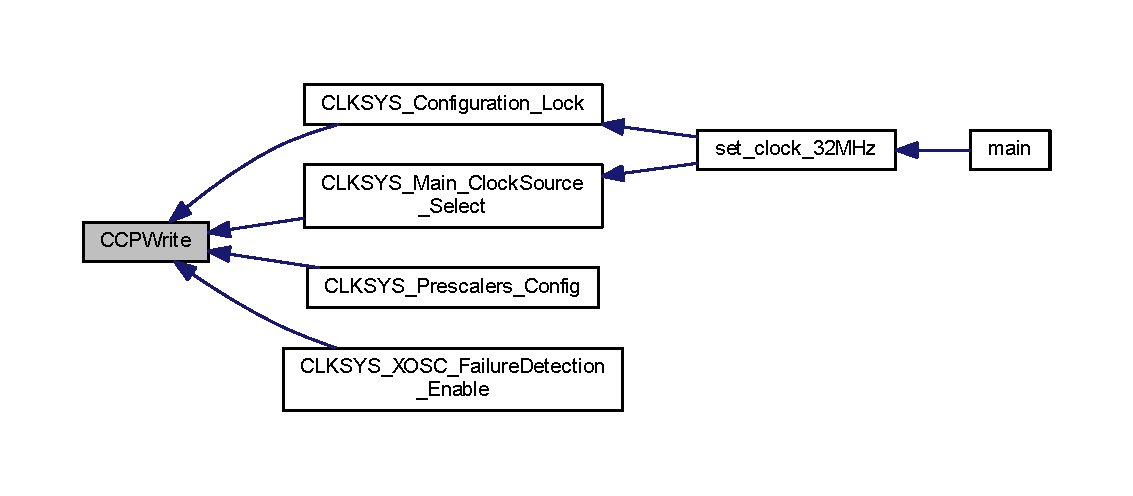
\includegraphics[width=350pt]{clksys__driver_8h_aad4e162434c2cc7e0087bbc0ddfe266c_icgraph}
\end{center}
\end{figure}
\hypertarget{clksys__driver_8h_a581c15c6c0b2eaa0c81f0b5cafc3b82d}{}\label{clksys__driver_8h_a581c15c6c0b2eaa0c81f0b5cafc3b82d} 
\index{clksys\+\_\+driver.\+h@{clksys\+\_\+driver.\+h}!C\+L\+K\+S\+Y\+S\+\_\+\+Auto\+Calibration\+\_\+\+Enable@{C\+L\+K\+S\+Y\+S\+\_\+\+Auto\+Calibration\+\_\+\+Enable}}
\index{C\+L\+K\+S\+Y\+S\+\_\+\+Auto\+Calibration\+\_\+\+Enable@{C\+L\+K\+S\+Y\+S\+\_\+\+Auto\+Calibration\+\_\+\+Enable}!clksys\+\_\+driver.\+h@{clksys\+\_\+driver.\+h}}
\subsubsection{\texorpdfstring{C\+L\+K\+S\+Y\+S\+\_\+\+Auto\+Calibration\+\_\+\+Enable()}{CLKSYS\_AutoCalibration\_Enable()}}
{\footnotesize\ttfamily void C\+L\+K\+S\+Y\+S\+\_\+\+Auto\+Calibration\+\_\+\+Enable (\begin{DoxyParamCaption}\item[{uint8\+\_\+t}]{clk\+Source,  }\item[{bool}]{ext\+Reference }\end{DoxyParamCaption})}



This function enables automatic calibration of the selected internal oscillator. 

Either the internal 32k\+Hz RC oscillator or an external 32k\+Hz crystal can be used as a calibration reference. The user must make sure that the selected reference is ready and running.


\begin{DoxyParams}{Parameters}
{\em clk\+Source} & Clock source to calibrate, either O\+S\+C\+\_\+\+R\+C2\+M\+C\+R\+E\+F\+\_\+bm or O\+S\+C\+\_\+\+R\+C32\+M\+C\+R\+E\+F\+\_\+gm -\/ patched to group mask(jb). \\
\hline
{\em ext\+Reference} & True if external crystal should be used as reference. \\
\hline
\end{DoxyParams}


Definition at line 260 of file clksys\+\_\+driver.\+c.



Referenced by set\+\_\+clock\+\_\+32\+M\+Hz().

Here is the caller graph for this function\+:\nopagebreak
\begin{figure}[H]
\begin{center}
\leavevmode
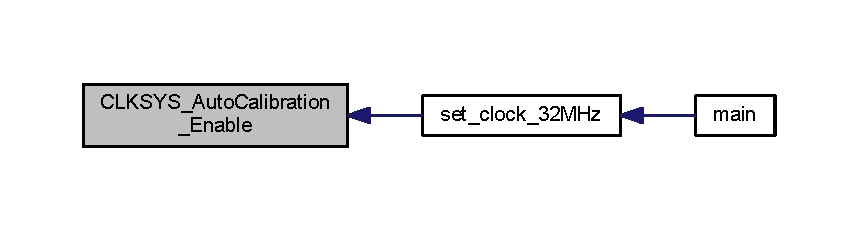
\includegraphics[width=350pt]{clksys__driver_8h_a581c15c6c0b2eaa0c81f0b5cafc3b82d_icgraph}
\end{center}
\end{figure}
\hypertarget{clksys__driver_8h_a6225fea8fc405c6d1dab88d0ad537173}{}\label{clksys__driver_8h_a6225fea8fc405c6d1dab88d0ad537173} 
\index{clksys\+\_\+driver.\+h@{clksys\+\_\+driver.\+h}!C\+L\+K\+S\+Y\+S\+\_\+\+Configuration\+\_\+\+Lock@{C\+L\+K\+S\+Y\+S\+\_\+\+Configuration\+\_\+\+Lock}}
\index{C\+L\+K\+S\+Y\+S\+\_\+\+Configuration\+\_\+\+Lock@{C\+L\+K\+S\+Y\+S\+\_\+\+Configuration\+\_\+\+Lock}!clksys\+\_\+driver.\+h@{clksys\+\_\+driver.\+h}}
\subsubsection{\texorpdfstring{C\+L\+K\+S\+Y\+S\+\_\+\+Configuration\+\_\+\+Lock()}{CLKSYS\_Configuration\_Lock()}}
{\footnotesize\ttfamily void C\+L\+K\+S\+Y\+S\+\_\+\+Configuration\+\_\+\+Lock (\begin{DoxyParamCaption}\item[{void}]{ }\end{DoxyParamCaption})}



This function lock the entire clock system configuration. 

This will lock the configuration until the next reset, or until the External Oscillator Failure Detections (X\+O\+S\+C\+FD) feature detects a failure and switches to internal 2\+M\+Hz RC oscillator. 

Definition at line 292 of file clksys\+\_\+driver.\+c.



References C\+C\+P\+Write().



Referenced by set\+\_\+clock\+\_\+32\+M\+Hz().

Here is the call graph for this function\+:\nopagebreak
\begin{figure}[H]
\begin{center}
\leavevmode
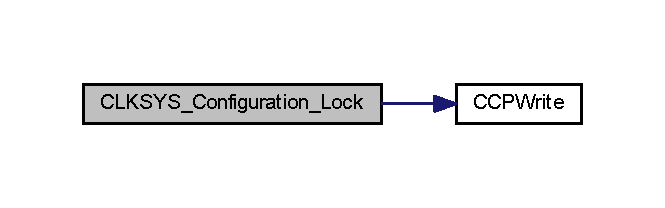
\includegraphics[width=319pt]{clksys__driver_8h_a6225fea8fc405c6d1dab88d0ad537173_cgraph}
\end{center}
\end{figure}
Here is the caller graph for this function\+:\nopagebreak
\begin{figure}[H]
\begin{center}
\leavevmode
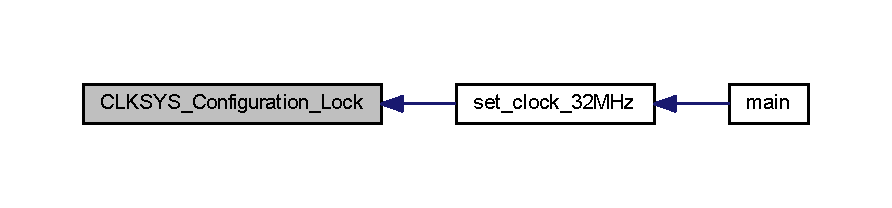
\includegraphics[width=350pt]{clksys__driver_8h_a6225fea8fc405c6d1dab88d0ad537173_icgraph}
\end{center}
\end{figure}
\hypertarget{clksys__driver_8h_a31b1ca1994b6a687974a119d1ad8008c}{}\label{clksys__driver_8h_a31b1ca1994b6a687974a119d1ad8008c} 
\index{clksys\+\_\+driver.\+h@{clksys\+\_\+driver.\+h}!C\+L\+K\+S\+Y\+S\+\_\+\+Disable@{C\+L\+K\+S\+Y\+S\+\_\+\+Disable}}
\index{C\+L\+K\+S\+Y\+S\+\_\+\+Disable@{C\+L\+K\+S\+Y\+S\+\_\+\+Disable}!clksys\+\_\+driver.\+h@{clksys\+\_\+driver.\+h}}
\subsubsection{\texorpdfstring{C\+L\+K\+S\+Y\+S\+\_\+\+Disable()}{CLKSYS\_Disable()}}
{\footnotesize\ttfamily uint8\+\_\+t C\+L\+K\+S\+Y\+S\+\_\+\+Disable (\begin{DoxyParamCaption}\item[{uint8\+\_\+t}]{osc\+Sel }\end{DoxyParamCaption})}



This function disables the selected oscillator. 

This function will disable the selected oscillator if possible. If it is currently used as a main system clock source, hardware will disregard the disable attempt, and this function will return zero. If it fails, change to another main system clock source and try again.


\begin{DoxyParams}{Parameters}
{\em osc\+Sel} & Bitmask of selected clock. Can be one of the following O\+S\+C\+\_\+\+R\+C2\+M\+E\+N\+\_\+bm, O\+S\+C\+\_\+\+R\+C32\+M\+E\+N\+\_\+bm, O\+S\+C\+\_\+\+R\+C32\+K\+E\+N\+\_\+bm, O\+S\+C\+\_\+\+X\+O\+S\+C\+E\+N\+\_\+bm, O\+S\+C\+\_\+\+P\+L\+L\+E\+N\+\_\+bm.\\
\hline
\end{DoxyParams}
\begin{DoxyReturn}{Returns}
Non-\/zero if oscillator was disabled successfully. 
\end{DoxyReturn}


Definition at line 187 of file clksys\+\_\+driver.\+c.



Referenced by set\+\_\+clock\+\_\+32\+M\+Hz().

Here is the caller graph for this function\+:\nopagebreak
\begin{figure}[H]
\begin{center}
\leavevmode
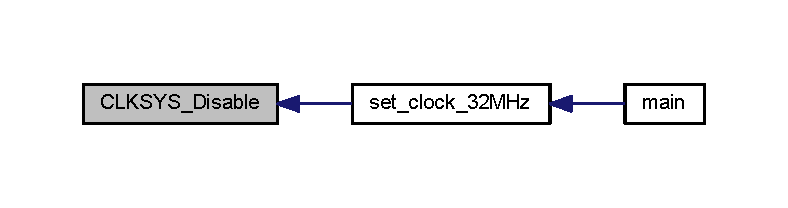
\includegraphics[width=350pt]{clksys__driver_8h_a31b1ca1994b6a687974a119d1ad8008c_icgraph}
\end{center}
\end{figure}
\hypertarget{clksys__driver_8h_a1e46c4a8f01a83d4e4747d32d113e7e2}{}\label{clksys__driver_8h_a1e46c4a8f01a83d4e4747d32d113e7e2} 
\index{clksys\+\_\+driver.\+h@{clksys\+\_\+driver.\+h}!C\+L\+K\+S\+Y\+S\+\_\+\+Main\+\_\+\+Clock\+Source\+\_\+\+Select@{C\+L\+K\+S\+Y\+S\+\_\+\+Main\+\_\+\+Clock\+Source\+\_\+\+Select}}
\index{C\+L\+K\+S\+Y\+S\+\_\+\+Main\+\_\+\+Clock\+Source\+\_\+\+Select@{C\+L\+K\+S\+Y\+S\+\_\+\+Main\+\_\+\+Clock\+Source\+\_\+\+Select}!clksys\+\_\+driver.\+h@{clksys\+\_\+driver.\+h}}
\subsubsection{\texorpdfstring{C\+L\+K\+S\+Y\+S\+\_\+\+Main\+\_\+\+Clock\+Source\+\_\+\+Select()}{CLKSYS\_Main\_ClockSource\_Select()}}
{\footnotesize\ttfamily uint8\+\_\+t C\+L\+K\+S\+Y\+S\+\_\+\+Main\+\_\+\+Clock\+Source\+\_\+\+Select (\begin{DoxyParamCaption}\item[{C\+L\+K\+\_\+\+S\+C\+L\+K\+S\+E\+L\+\_\+t}]{clock\+Source }\end{DoxyParamCaption})}



This function selects the main system clock source. 

Hardware will disregard any attempts to select a clock source that is not enabled or not stable. If the change fails, make sure the source is ready and running and try again.


\begin{DoxyParams}{Parameters}
{\em clock\+Source} & Clock source to use as input for the system clock prescaler block.\\
\hline
\end{DoxyParams}
\begin{DoxyReturn}{Returns}
Non-\/zero if change was successful. 
\end{DoxyReturn}


Definition at line 225 of file clksys\+\_\+driver.\+c.



References C\+C\+P\+Write().



Referenced by set\+\_\+clock\+\_\+32\+M\+Hz().

Here is the call graph for this function\+:\nopagebreak
\begin{figure}[H]
\begin{center}
\leavevmode
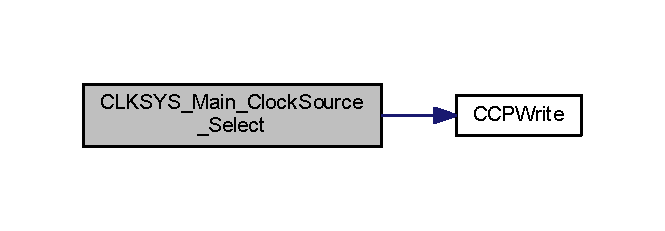
\includegraphics[width=319pt]{clksys__driver_8h_a1e46c4a8f01a83d4e4747d32d113e7e2_cgraph}
\end{center}
\end{figure}
Here is the caller graph for this function\+:\nopagebreak
\begin{figure}[H]
\begin{center}
\leavevmode
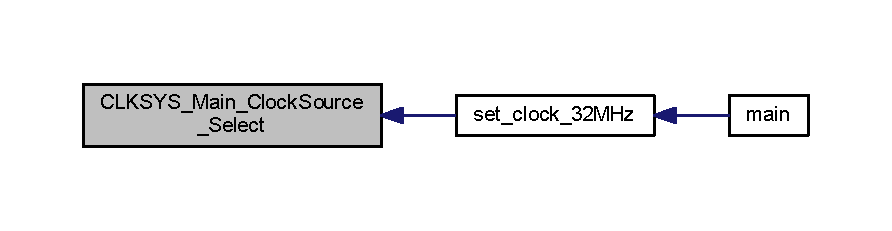
\includegraphics[width=350pt]{clksys__driver_8h_a1e46c4a8f01a83d4e4747d32d113e7e2_icgraph}
\end{center}
\end{figure}
\hypertarget{clksys__driver_8h_acb82744003806825da7fb6a7bb973941}{}\label{clksys__driver_8h_acb82744003806825da7fb6a7bb973941} 
\index{clksys\+\_\+driver.\+h@{clksys\+\_\+driver.\+h}!C\+L\+K\+S\+Y\+S\+\_\+\+P\+L\+L\+\_\+\+Config@{C\+L\+K\+S\+Y\+S\+\_\+\+P\+L\+L\+\_\+\+Config}}
\index{C\+L\+K\+S\+Y\+S\+\_\+\+P\+L\+L\+\_\+\+Config@{C\+L\+K\+S\+Y\+S\+\_\+\+P\+L\+L\+\_\+\+Config}!clksys\+\_\+driver.\+h@{clksys\+\_\+driver.\+h}}
\subsubsection{\texorpdfstring{C\+L\+K\+S\+Y\+S\+\_\+\+P\+L\+L\+\_\+\+Config()}{CLKSYS\_PLL\_Config()}}
{\footnotesize\ttfamily void C\+L\+K\+S\+Y\+S\+\_\+\+P\+L\+L\+\_\+\+Config (\begin{DoxyParamCaption}\item[{O\+S\+C\+\_\+\+P\+L\+L\+S\+R\+C\+\_\+t}]{clock\+Source,  }\item[{uint8\+\_\+t}]{factor }\end{DoxyParamCaption})}



This function configures the internal high-\/frequency P\+LL. 

Configuration of the internal high-\/frequency P\+LL to the correct values. It is used to define the input of the P\+LL and the factor of multiplication of the input clock source.

\begin{DoxyNote}{Note}
Note that the oscillator cannot be used as a main system clock source without being enabled and stable first. Check the ready flag before using the clock. The macro \hyperlink{clksys__driver_8h_a2cd92dbb89e4051b9385a61273d19dc6}{C\+L\+K\+S\+Y\+S\+\_\+\+Is\+Ready( \+\_\+osc\+Sel )} can be used to check this.
\end{DoxyNote}

\begin{DoxyParams}{Parameters}
{\em clock\+Source} & Reference clock source for the P\+LL, must be above 0.\+4\+M\+Hz. \\
\hline
{\em factor} & P\+LL multiplication factor, must be from 1 to 31, inclusive. \\
\hline
\end{DoxyParams}


Definition at line 167 of file clksys\+\_\+driver.\+c.

\hypertarget{clksys__driver_8h_a8e350b689dc409a4c9b902a192d1e8a3}{}\label{clksys__driver_8h_a8e350b689dc409a4c9b902a192d1e8a3} 
\index{clksys\+\_\+driver.\+h@{clksys\+\_\+driver.\+h}!C\+L\+K\+S\+Y\+S\+\_\+\+Prescalers\+\_\+\+Config@{C\+L\+K\+S\+Y\+S\+\_\+\+Prescalers\+\_\+\+Config}}
\index{C\+L\+K\+S\+Y\+S\+\_\+\+Prescalers\+\_\+\+Config@{C\+L\+K\+S\+Y\+S\+\_\+\+Prescalers\+\_\+\+Config}!clksys\+\_\+driver.\+h@{clksys\+\_\+driver.\+h}}
\subsubsection{\texorpdfstring{C\+L\+K\+S\+Y\+S\+\_\+\+Prescalers\+\_\+\+Config()}{CLKSYS\_Prescalers\_Config()}}
{\footnotesize\ttfamily void C\+L\+K\+S\+Y\+S\+\_\+\+Prescalers\+\_\+\+Config (\begin{DoxyParamCaption}\item[{C\+L\+K\+\_\+\+P\+S\+A\+D\+I\+V\+\_\+t}]{P\+S\+Afactor,  }\item[{C\+L\+K\+\_\+\+P\+S\+B\+C\+D\+I\+V\+\_\+t}]{P\+S\+B\+Cfactor }\end{DoxyParamCaption})}



This function changes the prescaler configuration. 

Change the configuration of the three system clock prescaler is one single operation. The user must make sure that the main C\+PU clock does not exceed recommended limits.


\begin{DoxyParams}{Parameters}
{\em P\+S\+Afactor} & Prescaler A division factor, O\+FF or 2 to 512 in powers of two. \\
\hline
{\em P\+S\+B\+Cfactor} & Prescaler B and C division factor, in the combination of (1,1), (1,2), (4,1) or (2,2). \\
\hline
\end{DoxyParams}


Definition at line 206 of file clksys\+\_\+driver.\+c.



References C\+C\+P\+Write().

Here is the call graph for this function\+:\nopagebreak
\begin{figure}[H]
\begin{center}
\leavevmode
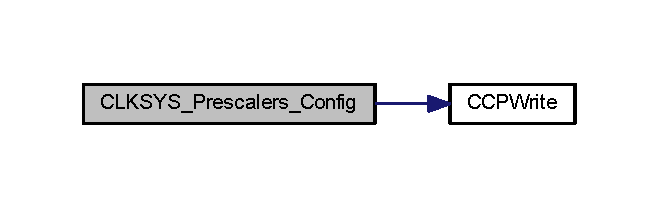
\includegraphics[width=316pt]{clksys__driver_8h_a8e350b689dc409a4c9b902a192d1e8a3_cgraph}
\end{center}
\end{figure}
\hypertarget{clksys__driver_8h_ae622e3056cd713fdca464b9fd6e5a7ab}{}\label{clksys__driver_8h_ae622e3056cd713fdca464b9fd6e5a7ab} 
\index{clksys\+\_\+driver.\+h@{clksys\+\_\+driver.\+h}!C\+L\+K\+S\+Y\+S\+\_\+\+R\+T\+C\+\_\+\+Clock\+Source\+\_\+\+Enable@{C\+L\+K\+S\+Y\+S\+\_\+\+R\+T\+C\+\_\+\+Clock\+Source\+\_\+\+Enable}}
\index{C\+L\+K\+S\+Y\+S\+\_\+\+R\+T\+C\+\_\+\+Clock\+Source\+\_\+\+Enable@{C\+L\+K\+S\+Y\+S\+\_\+\+R\+T\+C\+\_\+\+Clock\+Source\+\_\+\+Enable}!clksys\+\_\+driver.\+h@{clksys\+\_\+driver.\+h}}
\subsubsection{\texorpdfstring{C\+L\+K\+S\+Y\+S\+\_\+\+R\+T\+C\+\_\+\+Clock\+Source\+\_\+\+Enable()}{CLKSYS\_RTC\_ClockSource\_Enable()}}
{\footnotesize\ttfamily void C\+L\+K\+S\+Y\+S\+\_\+\+R\+T\+C\+\_\+\+Clock\+Source\+\_\+\+Enable (\begin{DoxyParamCaption}\item[{C\+L\+K\+\_\+\+R\+T\+C\+S\+R\+C\+\_\+t}]{clock\+Source }\end{DoxyParamCaption})}



This function selects a Real-\/\+Time Counter clock source. 

Selects the clock source for use by the Real-\/\+Time Counter (R\+TC) and enables clock signal routing to the R\+TC module.


\begin{DoxyParams}{Parameters}
{\em clock\+Source} & Clock source to use for the R\+TC. \\
\hline
\end{DoxyParams}


Definition at line 241 of file clksys\+\_\+driver.\+c.

\hypertarget{clksys__driver_8h_ace371b352e90117520436eb125aeeec0}{}\label{clksys__driver_8h_ace371b352e90117520436eb125aeeec0} 
\index{clksys\+\_\+driver.\+h@{clksys\+\_\+driver.\+h}!C\+L\+K\+S\+Y\+S\+\_\+\+X\+O\+S\+C\+\_\+\+Config@{C\+L\+K\+S\+Y\+S\+\_\+\+X\+O\+S\+C\+\_\+\+Config}}
\index{C\+L\+K\+S\+Y\+S\+\_\+\+X\+O\+S\+C\+\_\+\+Config@{C\+L\+K\+S\+Y\+S\+\_\+\+X\+O\+S\+C\+\_\+\+Config}!clksys\+\_\+driver.\+h@{clksys\+\_\+driver.\+h}}
\subsubsection{\texorpdfstring{C\+L\+K\+S\+Y\+S\+\_\+\+X\+O\+S\+C\+\_\+\+Config()}{CLKSYS\_XOSC\_Config()}}
{\footnotesize\ttfamily void C\+L\+K\+S\+Y\+S\+\_\+\+X\+O\+S\+C\+\_\+\+Config (\begin{DoxyParamCaption}\item[{O\+S\+C\+\_\+\+F\+R\+Q\+R\+A\+N\+G\+E\+\_\+t}]{freq\+Range,  }\item[{bool}]{low\+Power32k\+Hz,  }\item[{O\+S\+C\+\_\+\+X\+O\+S\+C\+S\+E\+L\+\_\+t}]{xosc\+Mode\+Selection }\end{DoxyParamCaption})}



This function configures the external oscillator. 

\begin{DoxyNote}{Note}
Note that the oscillator cannot be used as a main system clock source without being enabled and stable first. Check the ready flag before using the clock. The macro \hyperlink{clksys__driver_8h_a2cd92dbb89e4051b9385a61273d19dc6}{C\+L\+K\+S\+Y\+S\+\_\+\+Is\+Ready( \+\_\+osc\+Sel )} can be used to check this.
\end{DoxyNote}

\begin{DoxyParams}{Parameters}
{\em freq\+Range} & Frequency range for high-\/frequency crystal, does not apply for external clock or 32k\+Hz crystals. \\
\hline
{\em low\+Power32k\+Hz} & True of high-\/quality watch crystals are used and low-\/power oscillator is desired. \\
\hline
{\em xosc\+Mode\+Selection} & Combined selection of oscillator type (or external clock) and startup times. \\
\hline
\end{DoxyParams}


Definition at line 141 of file clksys\+\_\+driver.\+c.

\hypertarget{clksys__driver_8h_abfb0da2d81736412af825d46e7e0cedb}{}\label{clksys__driver_8h_abfb0da2d81736412af825d46e7e0cedb} 
\index{clksys\+\_\+driver.\+h@{clksys\+\_\+driver.\+h}!C\+L\+K\+S\+Y\+S\+\_\+\+X\+O\+S\+C\+\_\+\+Failure\+Detection\+\_\+\+Enable@{C\+L\+K\+S\+Y\+S\+\_\+\+X\+O\+S\+C\+\_\+\+Failure\+Detection\+\_\+\+Enable}}
\index{C\+L\+K\+S\+Y\+S\+\_\+\+X\+O\+S\+C\+\_\+\+Failure\+Detection\+\_\+\+Enable@{C\+L\+K\+S\+Y\+S\+\_\+\+X\+O\+S\+C\+\_\+\+Failure\+Detection\+\_\+\+Enable}!clksys\+\_\+driver.\+h@{clksys\+\_\+driver.\+h}}
\subsubsection{\texorpdfstring{C\+L\+K\+S\+Y\+S\+\_\+\+X\+O\+S\+C\+\_\+\+Failure\+Detection\+\_\+\+Enable()}{CLKSYS\_XOSC\_FailureDetection\_Enable()}}
{\footnotesize\ttfamily void C\+L\+K\+S\+Y\+S\+\_\+\+X\+O\+S\+C\+\_\+\+Failure\+Detection\+\_\+\+Enable (\begin{DoxyParamCaption}\item[{void}]{ }\end{DoxyParamCaption})}



This function enables the External Oscillator Failure Detection (X\+O\+S\+C\+FD) feature. 

The feature will stay enabled until next reset. Note that the X\+O\+S\+C\+FD {\itshape will} issue the X\+O\+S\+CF Non-\/maskable Interrupt (N\+MI) regardless of any interrupt priorities and settings. Therefore, make sure that a handler is implemented for the X\+O\+S\+CF N\+MI when you enable it. 

Definition at line 280 of file clksys\+\_\+driver.\+c.



References C\+C\+P\+Write().

Here is the call graph for this function\+:\nopagebreak
\begin{figure}[H]
\begin{center}
\leavevmode
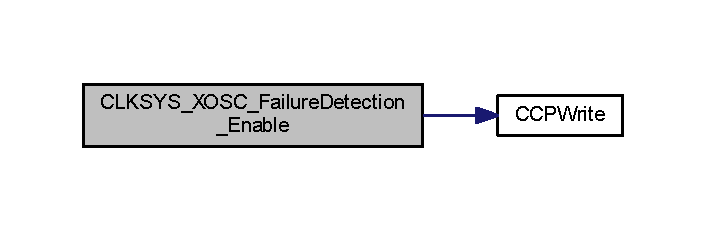
\includegraphics[width=339pt]{clksys__driver_8h_abfb0da2d81736412af825d46e7e0cedb_cgraph}
\end{center}
\end{figure}

\hypertarget{clock_8c}{}\section{clock.\+c File Reference}
\label{clock_8c}\index{clock.\+c@{clock.\+c}}


This file contains the Function to init, calibrate and change the clock.  


{\ttfamily \#include \char`\"{}clock.\+h\char`\"{}}\newline
Include dependency graph for clock.\+c\+:\nopagebreak
\begin{figure}[H]
\begin{center}
\leavevmode
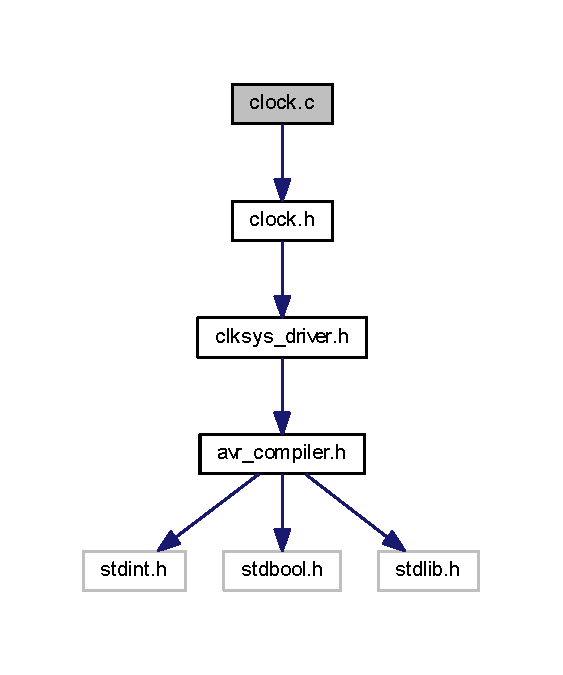
\includegraphics[width=270pt]{clock_8c__incl}
\end{center}
\end{figure}
\subsection*{Macros}
\begin{DoxyCompactItemize}
\item 
\#define \hyperlink{clock_8c_a43bafb28b29491ec7f871319b5a3b2f8}{F\+\_\+\+C\+PU}~32000000\+UL
\end{DoxyCompactItemize}
\subsection*{Functions}
\begin{DoxyCompactItemize}
\item 
void \hyperlink{clock_8c_a23a363c676847b1b84e6149472897fa2}{set\+\_\+clock\+\_\+32\+M\+Hz} (void)
\begin{DoxyCompactList}\small\item\em This function inits, calibrates and changes the clock. \end{DoxyCompactList}\end{DoxyCompactItemize}


\subsection{Detailed Description}
This file contains the Function to init, calibrate and change the clock. 

\begin{DoxyAuthor}{Author}
Jan Baudis 
\end{DoxyAuthor}
\begin{DoxyDate}{Date}
11.\+09.\+2016 14\+:24\+:30 
\end{DoxyDate}


\subsection{Macro Definition Documentation}
\hypertarget{clock_8c_a43bafb28b29491ec7f871319b5a3b2f8}{}\label{clock_8c_a43bafb28b29491ec7f871319b5a3b2f8} 
\index{clock.\+c@{clock.\+c}!F\+\_\+\+C\+PU@{F\+\_\+\+C\+PU}}
\index{F\+\_\+\+C\+PU@{F\+\_\+\+C\+PU}!clock.\+c@{clock.\+c}}
\subsubsection{\texorpdfstring{F\+\_\+\+C\+PU}{F\_CPU}}
{\footnotesize\ttfamily \#define F\+\_\+\+C\+PU~32000000\+UL}



\subsection{Function Documentation}
\hypertarget{clock_8c_a23a363c676847b1b84e6149472897fa2}{}\label{clock_8c_a23a363c676847b1b84e6149472897fa2} 
\index{clock.\+c@{clock.\+c}!set\+\_\+clock\+\_\+32\+M\+Hz@{set\+\_\+clock\+\_\+32\+M\+Hz}}
\index{set\+\_\+clock\+\_\+32\+M\+Hz@{set\+\_\+clock\+\_\+32\+M\+Hz}!clock.\+c@{clock.\+c}}
\subsubsection{\texorpdfstring{set\+\_\+clock\+\_\+32\+M\+Hz()}{set\_clock\_32MHz()}}
{\footnotesize\ttfamily void set\+\_\+clock\+\_\+32\+M\+Hz (\begin{DoxyParamCaption}\item[{void}]{ }\end{DoxyParamCaption})}



This function inits, calibrates and changes the clock. 

It enables the 32k\+Hz ref Clock for the Autocalibration and also executes the calibration. Afterwards it enables and changes to the 32\+M\+Hz internal Clock and also disables the 2\+M\+Hz \& 32k\+Hz clocks. Eventually it Locks the current Clock config. 

Definition at line 16 of file clock.\+c.



References C\+L\+K\+S\+Y\+S\+\_\+\+Auto\+Calibration\+\_\+\+Enable(), C\+L\+K\+S\+Y\+S\+\_\+\+Configuration\+\_\+\+Lock(), C\+L\+K\+S\+Y\+S\+\_\+\+Disable(), C\+L\+K\+S\+Y\+S\+\_\+\+Enable, C\+L\+K\+S\+Y\+S\+\_\+\+Is\+Ready, and C\+L\+K\+S\+Y\+S\+\_\+\+Main\+\_\+\+Clock\+Source\+\_\+\+Select().



Referenced by main().

Here is the call graph for this function\+:\nopagebreak
\begin{figure}[H]
\begin{center}
\leavevmode
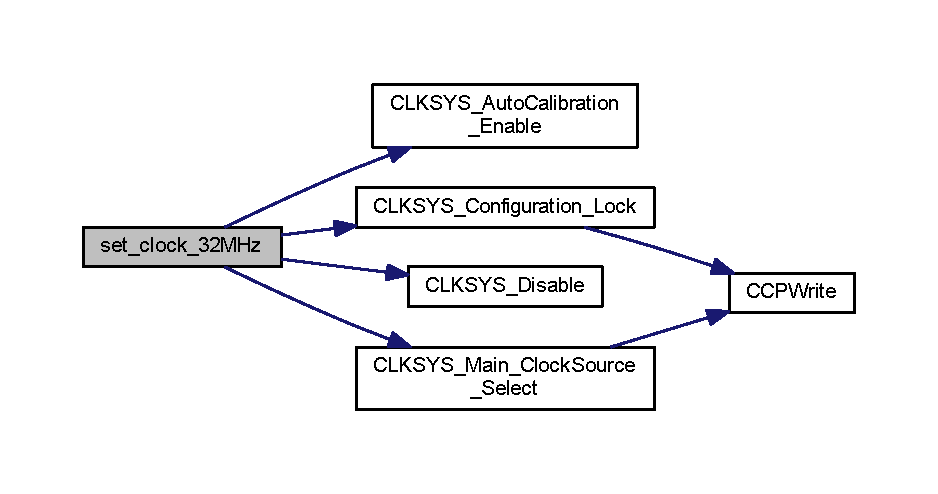
\includegraphics[width=350pt]{clock_8c_a23a363c676847b1b84e6149472897fa2_cgraph}
\end{center}
\end{figure}
Here is the caller graph for this function\+:\nopagebreak
\begin{figure}[H]
\begin{center}
\leavevmode
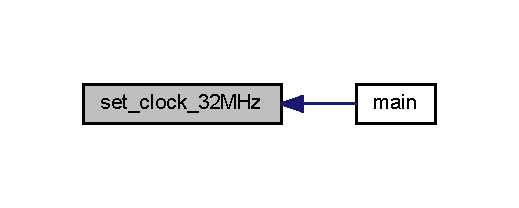
\includegraphics[width=249pt]{clock_8c_a23a363c676847b1b84e6149472897fa2_icgraph}
\end{center}
\end{figure}

\hypertarget{clock_8h}{}\section{clock.\+h File Reference}
\label{clock_8h}\index{clock.\+h@{clock.\+h}}


This file is the Headerfile for the clock-\/\+File. It contains the prototypes of the functions and the usual macros.  


{\ttfamily \#include \char`\"{}clksys\+\_\+driver.\+h\char`\"{}}\newline
Include dependency graph for clock.\+h\+:\nopagebreak
\begin{figure}[H]
\begin{center}
\leavevmode
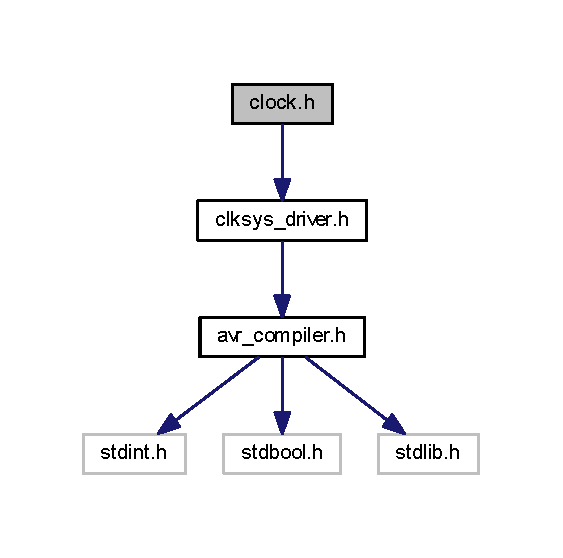
\includegraphics[width=270pt]{clock_8h__incl}
\end{center}
\end{figure}
This graph shows which files directly or indirectly include this file\+:\nopagebreak
\begin{figure}[H]
\begin{center}
\leavevmode
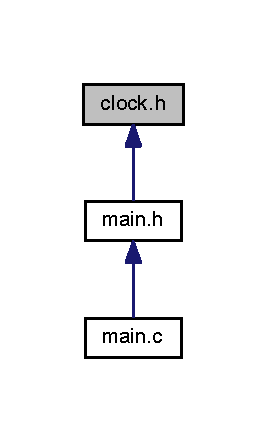
\includegraphics[width=192pt]{clock_8h__dep__incl}
\end{center}
\end{figure}
\subsection*{Functions}
\begin{DoxyCompactItemize}
\item 
void \hyperlink{clock_8h_a23a363c676847b1b84e6149472897fa2}{set\+\_\+clock\+\_\+32\+M\+Hz} (void)
\begin{DoxyCompactList}\small\item\em This function inits, calibrates and changes the clock. \end{DoxyCompactList}\end{DoxyCompactItemize}


\subsection{Detailed Description}
This file is the Headerfile for the clock-\/\+File. It contains the prototypes of the functions and the usual macros. 

\begin{DoxyAuthor}{Author}
Jan Baudis 
\end{DoxyAuthor}
\begin{DoxyDate}{Date}
11.\+09.\+2016 14\+:24\+:45 
\end{DoxyDate}


\subsection{Function Documentation}
\hypertarget{clock_8h_a23a363c676847b1b84e6149472897fa2}{}\label{clock_8h_a23a363c676847b1b84e6149472897fa2} 
\index{clock.\+h@{clock.\+h}!set\+\_\+clock\+\_\+32\+M\+Hz@{set\+\_\+clock\+\_\+32\+M\+Hz}}
\index{set\+\_\+clock\+\_\+32\+M\+Hz@{set\+\_\+clock\+\_\+32\+M\+Hz}!clock.\+h@{clock.\+h}}
\subsubsection{\texorpdfstring{set\+\_\+clock\+\_\+32\+M\+Hz()}{set\_clock\_32MHz()}}
{\footnotesize\ttfamily void set\+\_\+clock\+\_\+32\+M\+Hz (\begin{DoxyParamCaption}\item[{void}]{ }\end{DoxyParamCaption})}



This function inits, calibrates and changes the clock. 

It enables the 32k\+Hz ref Clock for the Autocalibration and also executes the calibration. Afterwards it enables and changes to the 32\+M\+Hz internal Clock and also disables the 2\+M\+Hz \& 32k\+Hz clocks. Eventually it Locks the current Clock config. 

Definition at line 16 of file clock.\+c.



References C\+L\+K\+S\+Y\+S\+\_\+\+Auto\+Calibration\+\_\+\+Enable(), C\+L\+K\+S\+Y\+S\+\_\+\+Configuration\+\_\+\+Lock(), C\+L\+K\+S\+Y\+S\+\_\+\+Disable(), C\+L\+K\+S\+Y\+S\+\_\+\+Enable, C\+L\+K\+S\+Y\+S\+\_\+\+Is\+Ready, and C\+L\+K\+S\+Y\+S\+\_\+\+Main\+\_\+\+Clock\+Source\+\_\+\+Select().



Referenced by main().

Here is the call graph for this function\+:\nopagebreak
\begin{figure}[H]
\begin{center}
\leavevmode
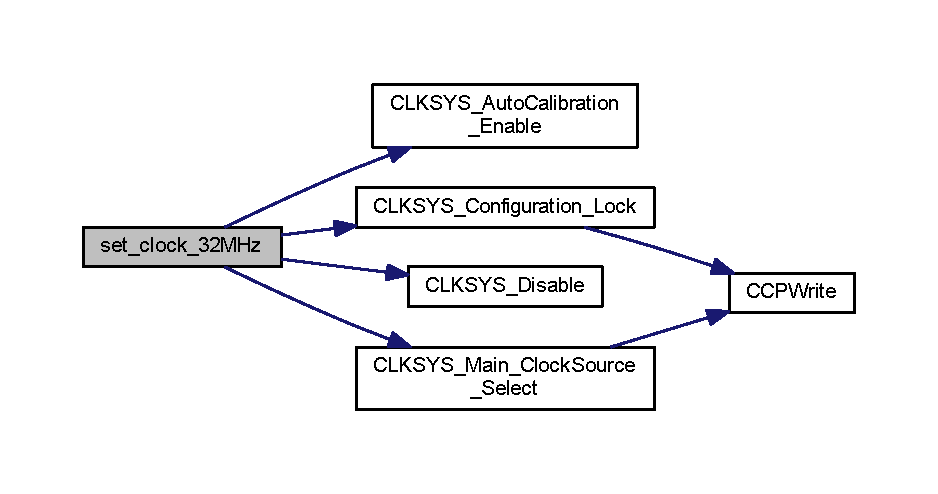
\includegraphics[width=350pt]{clock_8h_a23a363c676847b1b84e6149472897fa2_cgraph}
\end{center}
\end{figure}
Here is the caller graph for this function\+:\nopagebreak
\begin{figure}[H]
\begin{center}
\leavevmode
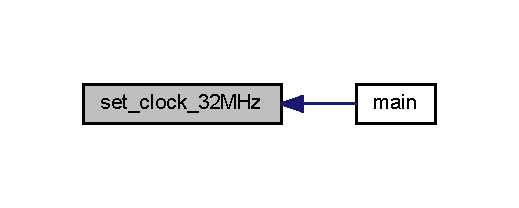
\includegraphics[width=249pt]{clock_8h_a23a363c676847b1b84e6149472897fa2_icgraph}
\end{center}
\end{figure}

\hypertarget{main_8c}{}\section{main.\+c File Reference}
\label{main_8c}\index{main.\+c@{main.\+c}}


This file is the main-\/\+File. It calls all the fancy Functions and so on.  


{\ttfamily \#include \char`\"{}main.\+h\char`\"{}}\newline
{\ttfamily \#include \char`\"{}U\+A\+R\+T.\+h\char`\"{}}\newline
Include dependency graph for main.\+c\+:
% FIG 0
\subsection*{Functions}
\begin{DoxyCompactItemize}
\item 
uint8\+\_\+t \hyperlink{main_8c_a69539018526f1fb80d3cf1c91bb08911}{U\+S\+A\+R\+T\+\_\+test} (\hyperlink{usart__driver_8h_a884c38d38327b0d4263c03cf0d84031e}{U\+S\+A\+R\+T\+\_\+data\+\_\+t} $\ast$usart\+\_\+data)
\item 
int \hyperlink{main_8c_a840291bc02cba5474a4cb46a9b9566fe}{main} (void)
\begin{DoxyCompactList}\small\item\em This is the main-\/\+Function. \end{DoxyCompactList}\end{DoxyCompactItemize}
\subsection*{Variables}
\begin{DoxyCompactItemize}
\item 
int volatile \hyperlink{main_8c_a37fd7702e47867237a1617ae4b4fab85}{ret\+\_\+pressed}
\end{DoxyCompactItemize}


\subsection{Detailed Description}
This file is the main-\/\+File. It calls all the fancy Functions and so on. 

\begin{DoxyAuthor}{Author}
Jan Baudis 
\end{DoxyAuthor}
\begin{DoxyDate}{Date}
08.\+09.\+2016 01\+:50\+:07 
\end{DoxyDate}


\subsection{Function Documentation}
\hypertarget{main_8c_a840291bc02cba5474a4cb46a9b9566fe}{}\label{main_8c_a840291bc02cba5474a4cb46a9b9566fe} 
\index{main.\+c@{main.\+c}!main@{main}}
\index{main@{main}!main.\+c@{main.\+c}}
\subsubsection{\texorpdfstring{main()}{main()}}
{\footnotesize\ttfamily int main (\begin{DoxyParamCaption}\item[{void}]{ }\end{DoxyParamCaption})}



This is the main-\/\+Function. 

It calls all the fancy Functions. It does things. Enter the \char`\"{}\+Shell\char`\"{}! 

Definition at line 29 of file main.\+c.



References enter\+\_\+shell(), receive\+\_\+string\+\_\+from\+\_\+usart(), ret\+\_\+pressed, send\+\_\+string\+\_\+pgm\+\_\+to\+\_\+usart(), send\+\_\+string\+\_\+to\+\_\+usart(), set\+\_\+clock\+\_\+32\+M\+Hz(), U\+S\+A\+R\+T\+\_\+\+D\+A\+T\+A\+\_\+\+PC, usart\+\_\+init\+\_\+pc(), and usart\+\_\+init\+\_\+tpuart().

Here is the call graph for this function\+:
% FIG 1
\hypertarget{main_8c_a69539018526f1fb80d3cf1c91bb08911}{}\label{main_8c_a69539018526f1fb80d3cf1c91bb08911} 
\index{main.\+c@{main.\+c}!U\+S\+A\+R\+T\+\_\+test@{U\+S\+A\+R\+T\+\_\+test}}
\index{U\+S\+A\+R\+T\+\_\+test@{U\+S\+A\+R\+T\+\_\+test}!main.\+c@{main.\+c}}
\subsubsection{\texorpdfstring{U\+S\+A\+R\+T\+\_\+test()}{USART\_test()}}
{\footnotesize\ttfamily uint8\+\_\+t U\+S\+A\+R\+T\+\_\+test (\begin{DoxyParamCaption}\item[{\hyperlink{usart__driver_8h_a884c38d38327b0d4263c03cf0d84031e}{U\+S\+A\+R\+T\+\_\+data\+\_\+t} $\ast$}]{usart\+\_\+data }\end{DoxyParamCaption})}



Definition at line 12 of file main.\+c.



References Usart\+\_\+and\+\_\+buffer\+::buffer, U\+S\+A\+R\+T\+\_\+\+Buffer\+::\+RX, and U\+S\+A\+R\+T\+\_\+\+Buffer\+::\+R\+X\+\_\+\+Tail.



\subsection{Variable Documentation}
\hypertarget{main_8c_a37fd7702e47867237a1617ae4b4fab85}{}\label{main_8c_a37fd7702e47867237a1617ae4b4fab85} 
\index{main.\+c@{main.\+c}!ret\+\_\+pressed@{ret\+\_\+pressed}}
\index{ret\+\_\+pressed@{ret\+\_\+pressed}!main.\+c@{main.\+c}}
\subsubsection{\texorpdfstring{ret\+\_\+pressed}{ret\_pressed}}
{\footnotesize\ttfamily int volatile ret\+\_\+pressed}



Definition at line 11 of file U\+A\+R\+T.\+c.



Referenced by main().


\hypertarget{main_8h}{}\section{main.\+h File Reference}
\label{main_8h}\index{main.\+h@{main.\+h}}


This file is the Headerfile for the main-\/\+File. It contains general things like the F\+\_\+\+C\+PU Macro etc.  


{\ttfamily \#include $<$avr/io.\+h$>$}\newline
{\ttfamily \#include \char`\"{}clksys\+\_\+driver.\+h\char`\"{}}\newline
{\ttfamily \#include \char`\"{}clock.\+h\char`\"{}}\newline
Include dependency graph for main.\+h\+:\nopagebreak
\begin{figure}[H]
\begin{center}
\leavevmode
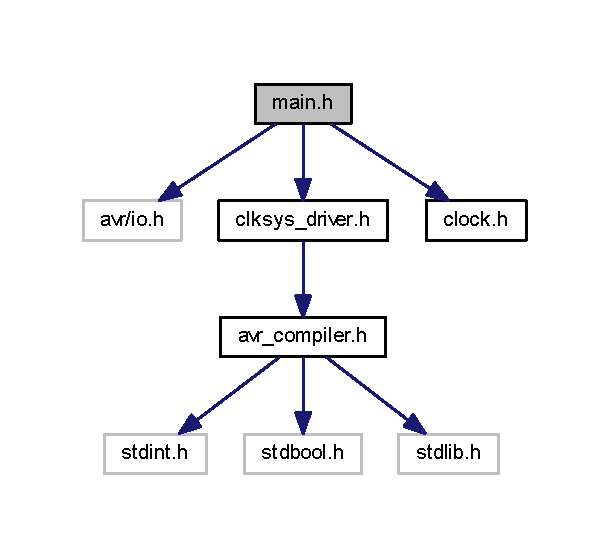
\includegraphics[width=293pt]{main_8h__incl}
\end{center}
\end{figure}
This graph shows which files directly or indirectly include this file\+:\nopagebreak
\begin{figure}[H]
\begin{center}
\leavevmode
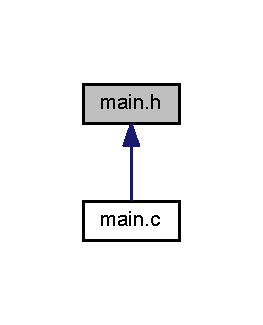
\includegraphics[width=126pt]{main_8h__dep__incl}
\end{center}
\end{figure}


\subsection{Detailed Description}
This file is the Headerfile for the main-\/\+File. It contains general things like the F\+\_\+\+C\+PU Macro etc. 

\begin{DoxyAuthor}{Author}
Jan Baudis 
\end{DoxyAuthor}

%--- End generated contents ---

% Index
\backmatter
\newpage
\phantomsection
\clearemptydoublepage
\addcontentsline{toc}{chapter}{Index}
\printindex

\end{document}
